%\usepackage{csquotes}%% !TeX program = lualatex

%\listfiles	
% **************************
% STOP - Bitte zuerst lesen, bevor Sie weitermachen
%
% Einige Dinge müssen Sie an Ihre Bedürfnisse (und die Vorgaben Ihres
% Betreuers anpassen. Editieren Sie dazu die Datei docinfo.tex).
%
% 1. Sprache
% Das Template unterstützt Deutsch und Englisch, Standard ist Deutsch.
% Wenn Sie Englisch verwenden wollen, ändern Sie bitte direkt am Anfang
% dieser Datei den Eintrag
%    \newcommand{\hsmasprache}{de}
% auf
%    \newcommand{\hsmasprache}{en}
%
% 2. Form der Abgabe
% Das Template unterstützt sowohl eine digitale Abgabe, als auch eine Abgabe
% auf Papier. Bei einer Papierabgabe wird ein doppelseitiger Druck vorbereitet
% und der Titel wird so platziert, dass er in das Fenster des offiziellen
% Umschlages der Technischen Hochschule passt.
% Bei einer digitalen Abgabe (als PDF) wird der Titel zentriert und als
% Format wird einseitig gewählt. Außerdem wird die Datei unterschrift.png
% auf dem Blatt mit der Erklärung zur Eigenständigkeit eingebunden.
%
% 3. Zitierstil
% Abhängig von dem gewünschten Zitierstil passen Sie bitte in
% hma.cls die Einstellungen bei \RequirePackage[backend=biber...
% an. Wie ist dort genau erklärt.
% Achtung: Wenn Sie als Zitierstil Fußnoten wählen bzw. generell
% -------  mit Fußnoten arbeiten, dann beachten Sie bitte, dass
%          Fußnoten in Bildunterschriften und Tabellenüberschriften
%          nicht funktionieren.
%          Siehe hierzu https://texfaq.org/FAQ-ftncapt
%          und https://texfaq.org/FAQ-footintab
%          Sinnvollerweise verzichten Sie auf Fußnoten an diesen
%          Stellen und fügen Quellen einfach per \parancite ein.
%
% 4. Doppelseitiger oder einseitiger Druck
% Das Template bestimmt, ob einseitig oder doppelseitig gedruckt wird
% anhand der Abgabeform (papier / digital). Wollen sie dies übersteuern,
% müssen Sie in der Datei preambel.tex folgende Zeile
% \KOMAoptions{twoside=true} für doppelsetigen Druck
% \KOMAoptions{twoside=false} für einsetigen Druck
% direkt vor \usepackage{xcolor} einsetzen. Prinzipiell sollten Sie aber
% das vorgeschlagene Format einfach so lassen.
%
% 5. Unnötige Teile entfernen
% Entfernen Sie die Teile, die Sie nicht brauchen, z.B. Anhänge
%
% 6. Silbentrennung
% LaTeX führt eine automatische Silbentrennung durch. Allerdings
% werden Wörter, die bereits einen Bindestrich enthalten nicht
% getrennt, z.B. Datenschutz-Grundverordnung. Wenn Sie Ihren Text auf
% Deutsch schreiben, können Sie dann alternativ "= für den Bindestrich
% im Wort verwenden, z.B. Datenschutz"=Grundverordnung, damit LaTeX
% weiterhin richtig trennt.
% Ist die Silbentrennung aus einem anderen Grund nicht erfolgt, sodass
% das Wort über den rechten Rand hinaussteht oder wenn Sie eine weitere
% Trennstelle wollen, können Sie LaTeX helfen, indem Sie weitere
% Trennstellen angeben. Dies geschieht durch "- als Zeichen, z.B.
% Staats"-vertrag.
%
% 7. Nummerierung der Fußnoten
% LaTeX beginnt die Nummerierung der Fußnoten in jedem Kapitel wieder
% bei 1. In diesem Template wird die fortlaufende Nummerierung der Fußnoten 
% über die gesamte Arbeit umgesetzt.  
%
% 8. Unterschrift
% Bei einer Abgabe auf Papier unterschreiben Sie die Arbeit eigenhändig.
% Geben Sie allerdings digital ab, sollten Sie die Datei unterschrift.png in dem 
% Ordner /bilder durch einen Scan Ihrer eigenen Unteschrift ersetzen - andernfalls
% unterschreiben Sie als Max Mustermann ;-)
% *******************************************************************


% Dokumenteneinstellungen und Infos importieren
% -------------------------------------------------------
% Informationen und Einstellungen für Ihre Abschlussarbeit
%

% Sprache für das Dokument festlegen
\newcommand{\hsmasprache}{de} %de für Deutsch oder en für Englisch


% Abgabeform festlegen
% Bei einer digitalen Abgabe, wird das Dokument einseitig erzeugt und der Titel wird
% zentriert.
\newcommand{\hsmaabgabe}{digital} % Abgabe erfolgt für Fakultät I digital. Optionen hier sind für anderen Fakultäten: "papier" oder "digital".


% Flags für Veröffentlichung, Sperrvermerk
\newcommand{\hsmapublizieren}{opensource}   
% Wird einer Veröffentlichung zugestimmt?
% Optionen: 
% opensource = Druck der CC Lizenz mit By SA (Standard)
% hs = Veröffentlichung an der Technischen Hochschule und auf Hochschulservern
% stud = kein opensource und keine veröffentlichung auf den Hochschulservern
% vertraulich = Arbeit darf nicht veröffentlicht werden und erhält einen Sperrvermerk (Nur nach Absprache mit Betreuer setzen!)


\newcommand{\genderhinweis}{gender}     % Soll der Gender-Hinweis angezeigt werden? ja=gender, nein = nogender; Genderhinweis wird nur in deutscher Sprache angezeigt!


\newcommand{\hsmaquellcode}{sourcecode} % Verwenden Sie Quellcode in Ihrer Arbeit? ja=sourcecode, nein= nosourcecode

\newcommand{\hsmasymbole}{symbole} % Verwenden Sie viele Symbole in Ihrer Arbeit, welche in einem Symbolverzeichnis aufgeführt werden sollen? ja=symbole, nein= nosymbole


\newcommand{\hsmaglossar}{glossar} % Verwenden Sie Begriffserklärungen nicht Abkürzungen in Ihrer Arbeit? ja=glossar, nein= noglossar

\newcommand{\hsmatc}{tc} % Verwenden der Änderungsmarkierung. Änderungsmarkierung aktiv und eine Liste der Änderungen wird angezeigt = tc, Keine Änderungsmarkierung und keine Ausgabe der Änderungen = notc




% Titel der Arbeit auf Deutsch
\newcommand{\hsmatitelde}{Copyright-Scanner: Automatisierte Erkennung und Extraktion von Copyright-Vermerken mittels Large Language Models. Konzeption, prototypische Implementierung und Evaluation eines Al-gestützten Analysetools im Lizenz-Compliance-Kontext.}
\newcommand{\hsmatiteldeabstract}{Copyright-Scanner: Automatisierte Erkennung und Extraktion von Copyright-Vermerken mittels Large Language Models. Konzeption, prototypische Implementierung und Evaluation eines Al-gestützten Analysetools im Lizenz-Compli- ance-Kontext.}

% Titel der Arbeit auf Englisch
\newcommand{\hsmatitelen}{Copyright Scanner: Automated Detection and Extraction of Copyright Notices Using Large Language Models. Design, Prototype Implementation, and Evaluation of an AI-Based Analysis Tool in the Context of License Compliance.}

% Weitere Informationen zur Arbeit
\newcommand{\hsmaort}{Mannheim}          % Ort
\newcommand{\hsmaautorvname}{Romeo Aljoscha Eren}        % Vorname(n)
\newcommand{\hsmaautornname}{Türemis} % Nachname(n)
\newcommand{\hsmaabgabedatum}{2025-08-31}% Datum der Abgabe in dem Format JJJJ-MM-TT

\newcommand{\hsmafirma}{Metaeffekt GmbH, Heidelberg} % Firma bei der die Arbeit durchgeführt wurde
\newcommand{\hsmabetreuer}{Prof. Dr. Sven-Gunnar Klaus, Technische Hochschule Mannheim} % Betreuer an der Hochschule
\newcommand{\hsmazweitkorrektor}{Karsten Klein, metaeffekt GmbH}   % Betreuer im Unternehmen oder Zweitkorrektor

\newcommand{\hsmafakultaet}{I}    % I für Informatik oder E, S, B, D, M, N, W, V
\newcommand{\hsmastudiengang}{IB} % IB IMB UIB CSB IM MTB (weitere siehe titleblatt.tex)


% Preambel importieren
% Dokumententyp, benutzte Pakete und deren Einstellungen
\documentclass[	\hsmasprache,%
				\hsmaabgabe,%
				\hsmapublizieren,%
				\genderhinweis,
				\hsmaquellcode,
				\hsmasymbole,
				\hsmaglossar,
				\hsmatc]{HMA}

% Wo sind die Bilder?
\graphicspath{{bilder/}}


% Wo liegt Sourcecode?
\newcommand{\srcloc}{src/}


% Checklisten mit zwei Ebenen
\newlist{checklist}{itemize}{2}
\setlist[checklist]{label=$\square$}



% Befehl zum Erstellen eigener Makros. In diesem Fall ist es ein Makro für das Einbinden von Bildern. Das label (für \ref) ist dann der Name der Bilddatei
\newcommand{\bild}[3]{
	\begin{figure}[ht]
		\centering
		\includegraphics[width=#2]{#1}
		\caption{#3}
		\label{#1}
\end{figure}}




							


\newcommand{\snowcard}[9]{
	\begin{table}[ht!]
		\caption{\hsmasnowcardanforderung\ #1 -- #4}\label{#1}
		\renewcommand{\arraystretch}{1.2}
		\centering
		\sffamily
		\begin{footnotesize}

			\begin{tabularx}{\linewidth}{sssssl}
				\toprule
				\textbf{\hsmasnowcardno} & #1 & \textbf{\hsmasnowcardart} & #2 & \textbf{\hsmasnowcardprio} & #3 \\
				\midrule
				\multicolumn{2}{l}{\textbf{\hsmasnowcardtitel}} & \multicolumn{4}{l}{\parbox[t]{11.8cm}{#4}} \\
				\ifx&#5&%
				\else
				\multicolumn{2}{l}{\textbf{\hsmasnowcardherkunft}} & \multicolumn{4}{l}{\parbox[t]{11.8cm}{#5}} \\
				\fi
				\ifx&#6&%
				\else
				\multicolumn{2}{l}{\textbf{\hsmasnowcardkonflikt}} & \multicolumn{4}{l}{\parbox[t]{11.8cm}{#6}} \\
				\fi
				\addlinespace
				\multicolumn{6}{l}{\textbf{\hsmasnowcardbeschreibung}} \\
				\multicolumn{6}{l}{\parbox[t]{13.5cm}{#7\strut}} \\
				\ifx&#8&%
				\else
				\addlinespace
				\multicolumn{6}{l}{\textbf{\hsmasnowcardfitkriterium}} \\
				\multicolumn{6}{l}{\parbox[t]{13.5cm}{#8\strut}} \\
				\fi
				\ifx&#9&%

				\else
				\addlinespace
				\multicolumn{6}{l}{\textbf{\hsmasnowcardmaterial}} \\
				\multicolumn{6}{l}{\parbox[t]{13.5cm}{#9\strut}} \\
				\fi
				\bottomrule
			\end{tabularx}
		\end{footnotesize}
	\end{table}
}



% Quality Attribute Scenario
\newcommand{\qas}[9]{
	\begin{table}[ht!]
		\caption{\hsmaqasanforderung\ #1 -- #3}\label{#1}
		\renewcommand{\arraystretch}{1.2}
		\centering
		\sffamily
		\begin{footnotesize}

			\begin{tabularx}{\linewidth}{sssssl}
				\toprule
				\textbf{\hsmaqasno} & #1 & \textbf{\hsmaqasart} & QAS & \textbf{\hsmaqasprio} & #2 \\
				\midrule
				\multicolumn{2}{l}{\textbf{\hsmaqastitel}} & \multicolumn{4}{l}{\parbox[t]{11.8cm}{#3}} \\
				\multicolumn{2}{l}{\textbf{\hsmaqasquelle}} & \multicolumn{4}{l}{\parbox[t]{11.8cm}{#4}} \\
				\multicolumn{2}{l}{\textbf{\hsmaqasstimulus}} & \multicolumn{4}{l}{\parbox[t]{11.8cm}{#5}} \\
				\multicolumn{2}{l}{\textbf{\hsmaqasartefakt}} & \multicolumn{4}{l}{\parbox[t]{11.8cm}{#6}} \\
				\addlinespace
				\multicolumn{6}{l}{\textbf{\hsmaqasumgebung}} \\
				\multicolumn{6}{l}{\parbox[t]{13.5cm}{#7\strut}} \\
				\addlinespace
				\multicolumn{6}{l}{\textbf{\hsmaqasantwort}} \\
				\multicolumn{6}{l}{\parbox[t]{13.5cm}{#8\strut}} \\
				\addlinespace
				\multicolumn{6}{l}{\textbf{\hsmaqasmass}} \\
				\multicolumn{6}{l}{\parbox[t]{13.5cm}{#9\strut}} \\
				\bottomrule
			\end{tabularx}
		\end{footnotesize}
	\end{table}
}




%Abstrakt Ihrer Abschlussarbeit
% -------------------------------------------------------
% Abstrakt / Abstract
% Achtung: Wenn Sie im Abstrakt Anführungszeichen verwenden wollen, dann benutzen Sie
%          nicht "` und "', sondern \enquote{}. "` und "' werden nicht richtig
%          erkannt.

% Kurze (maximal halbseitige) Beschreibung, worum es in der Arbeit geht auf Deutsch
\newcommand{\hsmaabstractde}{Jemand musste Josef K. verleumdet haben, denn ohne dass er etwas Böses getan hätte, wurde er eines Morgens verhaftet. Wie ein Hund! sagte er, es war, als sollte die Scham ihn überleben. Als Gregor Samsa eines Morgens aus unruhigen Träumen erwachte, fand er sich in seinem Bett zu einem ungeheueren Ungeziefer verwandelt. Und es war ihnen wie eine Bestätigung ihrer neuen Träume und guten Absichten, als am Ziele ihrer Fahrt die Tochter als erste sich erhob und ihren jungen Körper dehnte. Es ist ein eigentümlicher Apparat, sagte der Offizier zu dem Forschungsreisenden und überblickte mit einem gewissermaßen bewundernden Blick den ihm doch wohl bekannten Apparat. Sie hätten noch ins Boot springen können, aber der Reisende hob ein schweres, geknotetes Tau vom Boden, drohte ihnen damit und hielt sie dadurch von dem Sprunge ab. In den letzten Jahrzehnten ist das Interesse an Künstlern sehr zurückgegangen. Aber sie überwanden sich, umdrängten den Käfig und wollten sich gar nicht fortrühren.}

% Kurze (maximal halbseitige) Beschreibung, worum es in der Arbeit geht auf Englisch
\newcommand{\hsmaabstracten}{The European languages are members of the same family. Their separate existence is a myth. For science, music, sport, etc, Europe uses the same vocabulary. The languages only differ in their grammar, their pronunciation and their most common words. Everyone realizes why a new common language would be desirable: one could refuse to pay expensive translators. To achieve this, it would be necessary to have uniform grammar, pronunciation and more common words. If several languages coalesce, the grammar of the resulting language is more simple and regular than that of the individual languages. The new common language will be more simple and regular than the existing European languages. It will be as simple as Occidental; in fact, it will be Occidental. To an English person, it will seem like simplified English, as a skeptical Cambridge friend of mine told me what Occidental is.}



% Literatur-Datenbank
\addbibresource{literatur.bib}   % BibLaTeX-Datei mit Literaturquellen einbinden


% Anfang des Dokuments
\begin{document}	


%Laden der Dateien mit Abkürzungen, Begriffserklärungen (Glossar), Symbole
% General
\newacronym{sca}{SCA}{Software Composition Analysis}
\newacronym{nlp}{NLP}{Natural Language Processing}
\newacronym{cli}{CLI}{Command Line Interface}
\newacronym{json}{JSON}{JavaScript Object Notation}
\newacronym{api}{API}{Application Programming Interface}
\newacronym{oss}{OSS}{Open Source Software}
\newacronym{urhg}{UrhG}{Urheberrechtsgesetz}
\newacronym{gpl}{GPL}{GNU General Public License}
\newacronym{wua}{WUA}{Welturheberrechtsabkommen}
\newacronym{rbü}{RBÜ}{Revidierte Berner Übereinkunft}

% Policy
\newacronym{cir}{CIR}{Copyright Identification Rule}
\newacronym{air}{AIR}{Author Identification Rule}
\newacronym{hir}{HIR}{Holder Identification Rule}
\newacronym[plural=CEPs, longplural=Copyright Extraction Policies]{cep}{CEP}{Copyright Extraction Policy}
\newacronym[plural=AEPs, longplural=Author Extraction Policies]{aep}{AEP}{Author Extraction Policy}
\newacronym[plural=HEPs, longplural=Holder Extraction Policies]{hep}{HEP}{Holder Extraction Policy}
\newacronym[plural=GEPs, longplural=General Extraction Policies]{gep}{GEP}{General Extraction Policy}

% LLMs
\newacronym[plural=LLMs, longplural=Large Language Models]{llm}{LLM}{Large Language Model}
\newacronym{ner}{NER}{Named Entity Recognition}
\newacronym{ie}{IE}{Information Extraction}
\newacronym{tp}{TP}{True Positive}
\newacronym{fp}{FP}{False Positive}
\newacronym{fn}{FN}{False Negative}

% metaeffekt
\newacronym{tmd}{TMD}{Terms Metadata}
% Glossareinträge
\newglossaryentry{glos:quantization}{name={Quantization}, description={beschreibt den Vorgang, bei dem die Genauigkeit von Modellgewichten reduziert wird, um das Modell kleiner und effizienter zu machen.}}
\newglossaryentry{glos:benchmark}{name={Benchmark}, description={ist ein standardisierter Test oder Vergleichswert, mit dem die Leistung, Qualität oder Effizienz von Systemen, Prozessen oder Produkten objektiv bewertet wird.}}
\newglossaryentry{glos:fine-tuning}{name={Fine-Tuning}, description={ist der Prozess, bei dem ein bereits vortrainiertes Modell mit zusätzlichen, spezifischen Daten nachtrainiert wird, um es besser auf bestimmte Aufgaben oder Anwendungsbereiche abzustimmen.}}


% Verzeichnis von Symbolen und Einheiten
\newglossaryentry{symb:Pi}{name=\ensuremath{\pi},
	description={Geometrical value},
	unit={},
	type=symbolslist}

\newglossaryentry{symb:energyconsump}{name=\ensuremath{P},
	description={Energy consumption},
	unit={\si{kW}},
	type=symbolslist}
	
	
\pagestyle{headings}
\tableofcontents


\mainmatter

%% Ihre Inhaltsdateien werden an dieser Stelle in das Dokument eingefügt
\chapter{Daten}\label{ch:daten}

Die Qualität und Eignung des Datensatzes zählen zu den entscheidenden Faktoren für den Erfolg empirischer Arbeiten im Feld der \glspl{llm}.
Insbesondere bei der Evaluierung durch Benchmarks sowie beim Fine-Tuning wirken sich Aufbau, Umfang und Relevanz der verwendeten Daten unmittelbar auf die Aussagekraft der Ergebnisse aus.
Vor diesem Hintergrund erläutert das folgende Kapitel zunächst die Auswahl der Datenquelle und beschreibt im Anschluss die systematische Erstellung des Ausgangsdatensatzes.
Darauf aufbauend wird der Prozess der Weiterverarbeitung und Aggregation dargestellt, der schließlich in einem strukturierten Evaluations- und Testdatensatz resultiert.
Dieser bildet die Grundlage für die in dieser Arbeit durchgeführten Untersuchungen und stellt zugleich ein zentrales Ergebnis der Forschung dar.

% ======================================================================================================================

% Hier wird beschrieben, welche Datenquelle ausgewählt wurde, warum sie ausgewählt wurde und welche Alternativen es gab.
\section{Wahl der Datenquelle}\label{sec:wahl-der-datenquelle}

Um einen Evaluations- und Testdatensatz zu erzeugen, muss zuerst eine geeignete Datenquelle identifiziert und gegen Alternativen abgewogen werden.
Die Datenquelle wird anhand folgender Anforderungen ausgewählt:

\begin{itemize}
    \item \textit{Verfügbarkeit} -- die Datenquelle muss für die metaeffekt frei zugänglich sein.
    \item \textit{Realitätsnähe} -- die Datenquelle muss heterogene, reale Daten enthalten, künstliche Daten sind zu vermeiden.
    \item \textit{Umfang} -- der Datensatz muss einen für den Anwendungsfall ausreichenden Umfang haben.
    \item \textit{Reproduzierbarkeit} -- der Datensatz soll durch einen reproduzierbaren Prozess erzeugt werden können.
    \item \textit{Erweiterbarkeit} -- der Datensatz soll durch zusätzliche Quellen erweiterbar sein.
\end{itemize}

% TODO: Quelle einfügen
Eine naheliegende Datenquelle ist das GitHub-Repository des ScanCode-Toolkits, welches einen Testdatensatz zur Erkennung von Copyrights beinhaltet.
Dieser Datensatz besteht aus Quellcode-Dateien und ihren zugehörigen ScanCode-Ergebnissen.
Der Datensatz ist, wie auch das ScanCode-Toolkit, frei verfügbar.
Da es sich in erster Linie um Testdaten für die bestehende Implementierung handelt, bestehen diese zum Teil aus künstlich erzeugten, kuratierten Testfällen.
Eine Unterscheidung zwischen realen und synthetischen Beispielen ist jedoch im Datensatz nicht explizit gegeben.
Es fehlen sowohl entsprechende Bezeichner als auch strukturelle Merkmale, die Rückschlüsse auf den Ursprung einzelner Datenpunkte zulassen.
Außerdem ist es schwer einzuschätzen, inwiefern die Testdaten ein reales Spektrum an Copyrights abdecken.
Jedoch ist der Umfang des Testdatensatzes mit mehreren Tausend Dateien ausreichend für die vorgesehene Verwendung (\gls{glos:benchmark} und \gls{glos:fine-tuning}).
Der Datensatz wurde manuell kuratiert und entspringt keinem wiederholbaren Prozess, eine Reproduzierbarkeit ist somit nicht gegeben.
Wegen des fehlenden Prozesses ist der Datensatz nur manuell um weitere Quellen erweiterbar.

Die Lizenzdatenbank der metaeffekt \gls{tmd} bietet sich ebenfalls als Datenquelle an.
Sie umfasst über \num{2728} Lizenztexte und ihre metaeffekt-interne Modellierung.
Die Lizenztexte enthalten zwar Copyright-Statements, allerdings dienen diese hauptsächlich als Randfälle, die zur Umsetzung der \nameref{subsec:cep-04} dienen können.
Sowohl eine verallgemeinerte Realitätsnähe, als auch die Reproduzierbarkeit und Erweiterbarkeit sind bei dieser Datenquelle kaum gegeben.

Im Laufe der Arbeit wurde mit einem durch die Prozesse der metaeffekt analysierten und inventarisierten Alpine-Linux-Container eine weitere Datenquelle identifiziert.
Diese beruht im Gegensatz zu den Testdaten des ScanCode-Toolkits nicht auf künstlichen, sondern ausschließlich auf realen Daten und übertrifft dessen Umfang um ein Vielfaches.
Der Container beinhaltet ein breites Spektrum an Paketen sowie Quellcode und ist als Produkt der metaeffekt-Werkzeuge direkt verfügbar.
Da das Scan-Ergebnis auf einem automatischen Prozess basiert, kann es jederzeit reproduziert und um weitere Scan-Ergebnisse von anderen Quellen erweitert werden.
Außerdem ist dieser Container durch seine komplexe Kombination aus zahlreichen, über Jahrzehnte gewachsenen Komponenten mit vielfältiger Urheberschaft ein angemessenes und repräsentatives Fallbeispiel für diese Forschung.

Anhand der genannten Anforderungen wurde der Alpine-Container-Scan als Datenquelle dieser Arbeit gewählt.
Die konkrete Erzeugung dieser Datenquelle wird im nächsten Abschnitt erläutert.

% ======================================================================================================================

\section{Erzeugung des Ausgangsdatensatzes}\label{sec:erzeugung-datensatz}

Beim Scan des Alpine-Containers mithilfe des metaeffekt-Scanners laufen mehrere Verarbeitungsschritte ab, die für die Aggregation eines Copyright-Datensatzes relevant sind.
Zunächst werden sämtliche Datenpakete entpackt und die resultierenden Quellcode-Dateien in eines oder mehrere Segmente unterteilt.
Die resultierenden Segmente werden normalisiert und auf diese normalisierten Segmente werden Scan-Prozesse, wie der ScanCode-Service, angewandt.

Das vom ScanCode-Service erzeugte Ergebnis enthält die ermittelten Copyright-Informationen für ein normalisiertes Segment.
Die Normalisierung umfasst unter anderem das Entfernen mehrfacher Leerzeichen sowie von Zeilenumbrüchen.
Die \nameref{subsec:cep-01} besagt, dass Copyright-Statements nicht verändert werden dürfen.
Da die Normalisierung und Segmentierung den originalen Zustand der Datei verändern, können sie nicht für den Datensatz herangezogen werden.
Stattdessen werden die in den Segmenten referenzierten Originaldateien ermittelt und für jede Datei die Scan-Ergebnisse aller ihrer Segmente zurückgeführt.

% TODO: Eventuell hier kurz darauf eingehen, dass der SHA-1 Hash gewählt wurde, um kollisionen zu vermeiden und von originalen Dateinamen zu abstrahieren. Wahrscheinlichkeit für Kollision nennen.
Um Namenskonflikte zu vermeiden, wurde für jede Originaldatei der SHA-1 Hash berechnet und zusammen mit dem Dateityp zur Benennung der Datei verwendet.
Da die Verzeichnisstruktur der Originaldateien nicht relevant ist, werden alle Dateien in einem flachen Verzeichnis gespeichert, dies vereinfacht die anschließende Verarbeitung zusätzlich.
Der resultierende Ausgangsdatensatz umfasst etwa \num{467000} Originaldateien und ihre Scan-Ergebnisse.

% ======================================================================================================================

\section{Analyse des Datensatzes und Kategorisierung der Daten}\label{sec:analyse-datensatz}

Der erzeugte Datensatz kann in seiner extrahierten Form noch nicht für Evaluation und Test verwendet werden, da die Scan-Ergebnisse nicht auf den Originaldateien, sondern auf ihren normalisierten Segmenten beruhen.
Um diese Problematik zu adressieren, muss ein Prozess bestimmt werden, der bereits korrekte Daten ermittelt und fehlerhafte Daten, sofern möglich, korrigiert.
Korrekt bedeutet in diesem Kontext, dass die extrahierten Daten der Policy entsprechen.
Dieser Prozess wird nachfolgend schrittweise beschrieben.

\paragraph{Schritt 1 -- Unterteilung nach ScanCode-Ergebnissen}
Der Datensatz wurde in zwei Kategorien unterteilt: Dateien, für die ScanCode \textit{copyrights}, \textit{holders} bzw. \textit{authors} ermitteln konnte, und solche, die keine der genannten Informationen enthalten.
Etwa zwei Drittel des Datensatzes gehören zur letzteren Kategorie.
Die Daten ohne ScanCode-Ergebnis sind allerdings dennoch relevant, da es sich hierbei um False-Negatives des ScanCode-Toolkit handeln kann, die zur Verbesserung der Extraktion unbedingt ermittelt werden müssen.

\paragraph{Schritt 2 -- Entfernung von Duplikaten}
Zunächst wurden Duplikate aus dem Datensatz mit ScanCode-Ergebnissen entfernt.
Hierzu wurden Daten mit demselben SHA-1 Hash ermittelt und alle Duplikate eliminiert.
Diese Filterung reduzierte den Datensatz um etwa 8\,\%.

\paragraph{Schritt 3 -- Trennung von Einträgen ohne Copyrights}
Der von Duplikaten bereinigte Datensatz wurde danach unterteilt, ob das ScanCode-Ergebnis ausschließlich \textit{authors} enthält.
% TODO: Kategorie von contains no copyrigths zu contains only authors umbenennen.
Diese Kategorie von Daten ohne Copyrights (\textit{only authors}) umfasst ca.\ 11\,000 Dateien und dient dazu, die Extraktion auf False-Positives beim Erkennen der \textit{copyrights} zu analysieren.
Außerdem kann dieser Datensatz genutzt werden, das Extrahieren von Autoren gezielt und isoliert zu untersuchen.

\paragraph{Schritt 4 -- Abgleich mit Originaldateien (\enquote{exact matches})}
Die extrahierten Copyright-Statements der ScanCode-Ergebnisse wurden in den entsprechenden Originaldateien gesucht.
Wenn eine Originaldatei jedes der extrahierten Statements exakt enthält, wurde diese Datei und ihr extrahiertes Ergebnis den \textit{exact matches} zugeordnet.
Das exakte Vorkommen des extrahierten Statements in der Originaldatei erfüllt die Bedingung einer Extraktion \enquote{as-is} gemäß \nameref{subsec:cep-01}.
ScanCode-Ergebnisse, die einen \textit{exact match} aufweisen und keine Blöcke von Copyrights beinhalten (siehe \nameref{subsec:cep-03}), sind demnach ohne weitere Verarbeitung in Hinsicht auf ihre \textit{copyrights} Policy-konform.
Blöcke von Copyright-Statements können zwar für jedes extrahierte Statement einen \textit{exact match} aufweisen, verstoßen aber durch ihre ScanCode bedingte Aufteilung gegen die \nameref{subsec:cep-03}.
Eine korrekte Extraktion der \textit{holders} und \textit{authors} erfordert komplexere Mechanismen und wird im Laufe der Arbeit hauptsächlich durch manuelle Überprüfung gewährleistet.
Da die Priorität bei einer korrekten Extraktion der \textit{copyrights} liegt, werden die möglicherweise fehlerhaft extrahierten Urheber und Autoren als akzeptable Fehlertoleranz hingenommen.

\paragraph{Schritt 5 -- Analyse und Rekonstruktion der \enquote{mismatches}}
Die ScanCode-Ergebnisse ohne \textit{exact match} umfassen ca.\ zwei Drittel des Datensatzes.
Die Analyse dieser Ergebnisse zeigte, dass ScanCode unter anderem die Groß- und Kleinschreibung der Statements normalisiert.
Ein Beispiel hierfür ist die konsequente Ersetzung der \enquote{(C)} Markierung durch \enquote{(c)}.
Um diese Fälle zu identifizieren, wurden alle Originaldateien und ihre ScanCode-Ergebnisse in Kleinbuchstaben umgewandelt und anschließend überprüft, ob für jedes extrahierte Statement ein \textit{exact match} vorliegt.
Wenn ein solcher Match vorlag, konnte geschlussfolgert werden, dass die einzige Differenz zwischen Originaldatei und Extrakt die Groß- bzw.\ Kleinschreibung war.
Dieser Teil des Datensatzes wurde der Kategorie \textit{case-insensitive matches} zugeordnet und die enthaltenen Fälle wurden anschließend zu \textit{exact matches} aufgewertet.
Die Rekonstruktion der Original-Statements erfolgte, indem das extrahierte Statement in der Originaldatei gesucht und anschließend das Original-Statement im Ergebnis ersetzt wurde.
Auf diese Weise konnten ca.\ \num{57000} Dateien den \textit{exact matches} hinzugefügt werden.

\paragraph{Schritt 6 -- Rekonstruktion der Formatierung}
Da sowohl durch das ScanCode-Toolkit als auch durch die metaeffekt Prozesse Normalisierungen stattfinden, gehen Formatierungen wie Zeilenumbrüche und Tabulatoren bzw.\ mehrfache Leerzeichen verloren.
Um die \nameref{subsec:cep-06} zu erfüllen, muss die Formatierung im extrahierten Copyright-Statement erhalten bleiben.
Die durch Normalisierung betroffenen Statements wurden dadurch identifiziert, dass aus den Originaldateien und ScanScode-Ergebnissen jegliche Formatierungen, also Leerzeichen, Zeilenumbrüche und Tabulatoren entfernt wurden.
Anschließend wurde überprüft, ob für jedes Statement einer Datei ein \textit{exact match} vorliegt.
Die Rekonstruktion dieser \textit{format-insensitive matches} erfordert, dass das Statement in der Originaldatei gefunden und anschließend in das ScanCode-Ergebnis kopiert wird.
Da die Statements durch ihre Formatierung nicht eindeutig dem Ergebnis zuweisbar sind, wurde die Levenstein-Distanz zwischen den extrahierten Statements und jedem Substring der Originaldatei berechnet und der Substring gewählt, welcher die geringste Distanz zum Statement ergab.
Anschließend wurden alle Zeichen zwischen dem ersten und letzten Index des Substring aus der Originaldatei in das ScanCode-Ergebnis übertragen.
Durch diese Methode konnten ca.\ \num{6000} \textit{case-insensitive matches} rekonstruiert werden.
Die Statements erfordern dennoch Teils manuelle Arbeit, da bei mehrzeiligen Statements die in Kommentarsyntax eingebettet sind, nun auch die entspreche Kommentarsyntax in die Metadaten übertagen wurde.

Die Kategorie \textit{case-and-format-insensitive-matches} enthält solche Fälle, die sowohl abweichende Formatierung als auch abweichende Groß- und Kleinschreibung im ScanCode-Ergebnis enthalten.
Die Fälle dieser Kategorie wurden dadurch ermittelt, dass zunächst jegliche Formatierung und dann jede Großschreibung in den Originaldateien und den ScanCode-Ergebnissen entfernt wurde, anschließend wurde auch \textit{exact matches} geprüft.
Von den ursprünglichen rund \num{94000} \textit{mismatches} gehören nach den vorherigen Schritten noch ca.\ \num{27000} Dateien der Kategorie \textit{unresolved mismatches} an.
Diese Kategorie erfordert weitere Untersuchungen und weitgehend manuelle Aufbereitung.

\paragraph{Schritt 7 -- Identifizierung von \enquote{multiple copyrights}}
Die \textit{exact matches} wurden danach unterteilt, ob das entsprechende ScanCode-Ergebnis mehrere oder nur ein einzelnes Statement beinhalten.
Die Dateien, welche mehrere Statements beinhalten wurden der Kategorie \textit{multiple copyrights} zugeordnet und anschließend erneut unterteilt, je nachdem ob sie \textit{authors} enthalten oder nicht.
Die Absicht bei der Unterteilung nach \textit{multiple copyrights} und die anschließende Unterteilung nach \textit{authors} soll dazu dienen, dass beim späteren Erstellen von Benchmark- bzw.\ Evaluationsdatensätzen möglichst viele Formen von Copyrights in vergleichbarer Anzahl vorhanden sind.

\paragraph{Schritt 8 -- Identifizierung von \enquote{single copyrights}}
Analog zu den \textit{multiple copyrights} wurden die \textit{single copyrights} identifiziert und nach dem Vorkommen von \textit{authors} unterteilt.
Die resultierenden Kategorien \textit{single copyrights with authors} und \textit{single copyrights without authors} sind die zwei größten Unterkategorien des Datensatzes mit ca.\ \num{20000} Dateien ohne und ca.\ \num{70000} Dateien mit \textit{authors}.

\paragraph{Schritt 9 -- Manuelle Datenpflege}
Im Laufe dieser Arbeit wurde zu mehreren Zeitpunkten eine Untermenge aller Kategorien manuell anhand der Policy geprüft und, wenn nötig, korrigiert.
Diese manuell gepflegten Daten wurden regelmäßig dem Stakeholder stichprobenartig zur Validierung vorgelegt und sofern Unregelmäßigkeiten identifiziert wurden, angepasst.
Diese Validierungsschritte trugen zusätzlich zur Schärfung der Policy bei.
Die manuelle Erstellung eines Datensatzes ist enorm zeitaufwändig.
Die Überlegenheit von \glspl{llm} die auf sorgfältig kuratierten Datensätzen trainiert wurden gegenüber z.B.\ generierten Daten oder \gls{glos:zero-shot}- bzw.\ \gls{glos:few-shot}-Ansätze zeigen mehrere Studien\autocite{breton_empowering_2024}\autocite{villena_llmner_2024}.
% TODO: hier die finale Zahl der manuellen Datenpflege eintragen und noch auf die Zusammensetzung pro Kategorie eingehen.
Der resultierende Datensatz \textit{manually checked} umfasst \num{700} Dateien und stellt die Kategorie mit der höchsten Qualität in Hinsicht auf die Policy dar.
Mithilfe dieses Datensatzes soll die Option untersucht werden, ein \gls{llm} durch Fine-Tuning für den Anwendungsfall zu spezialisieren.

\begin{figure}[ht]
    \centering
    \makebox[\textwidth]{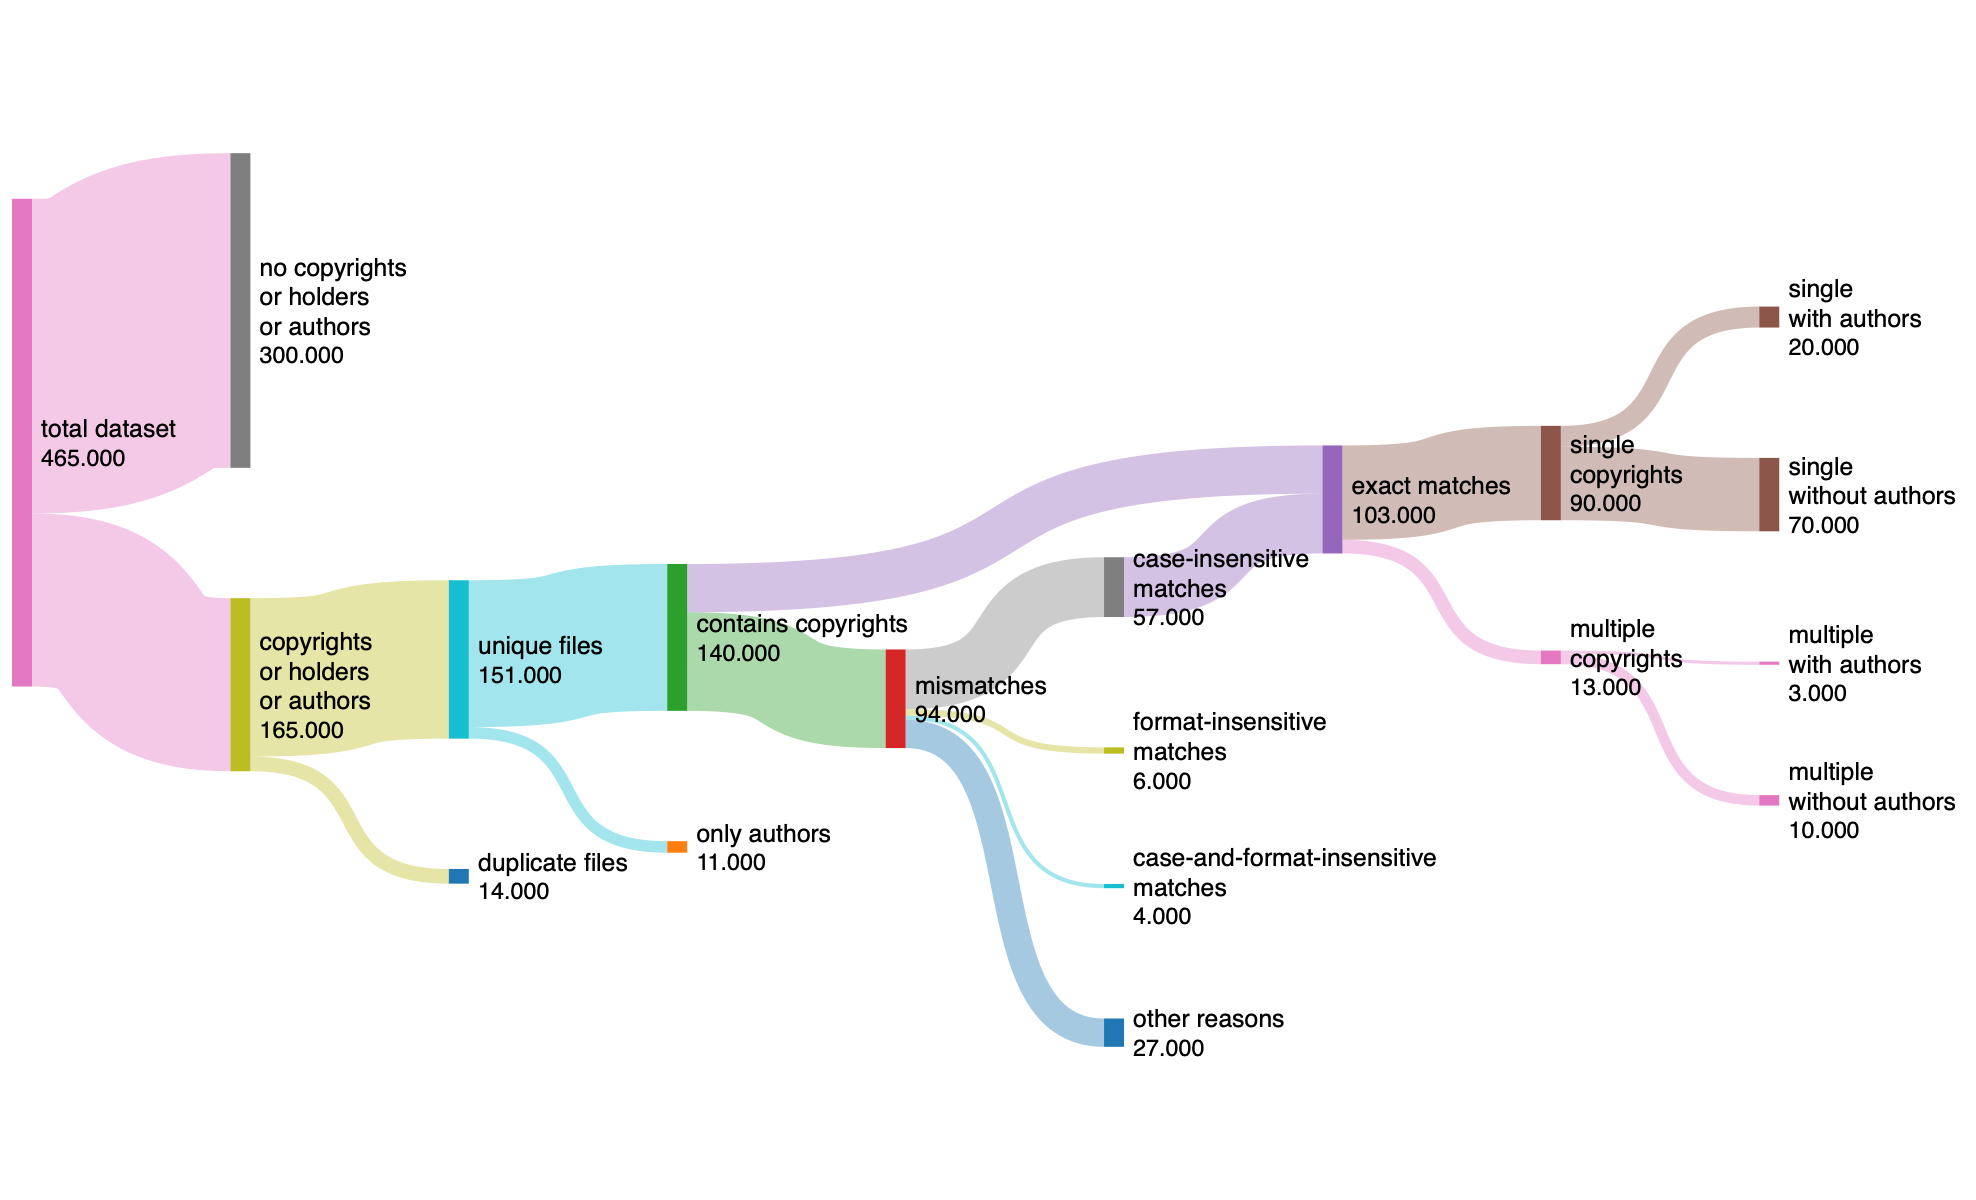
\includegraphics[width=1.3\textwidth]{daten/data-sankey}}
    \caption{
Sankey-Diagramm der Kategorien extrahierter Copyright-Informationen bei der Datenaggregation. Die Darstellung zeigt die schrittweise Reduktion und Klassifikation von \num{465000} Quellcodedateien entlang von Kriterien wie Duplikaterkennung, Copyright-Extraktion, Übereinstimmungsgrad mit den Originaldateien sowie Autorenerkennung. Die Breite der Flüsse entspricht der jeweiligen Anzahl an Dateien pro Kategorie.}
    \label{fig:data-sankey}
\end{figure}
Das Resultat der Datenaggregation sind zehn Hauptkategorien von Dateien, welche unterschiedliche Qualitätsstufen in Hinsicht auf die Policy und auf den Aufwand in ihrer Nachbereitung aufweisen.
Die \autoref{fig:data-sankey} veranschaulicht die schrittweise Verarbeitung und Kategorisierung der Daten.
Besonders bei der Abbildung hervorzuheben ist die Zusammenführung der \textit{exact matches} und der rekonstruierten \textit{case-insensitive matches}, welche den größten Anteil des Datensatzes ausmachen.
Die aggregierten Kategorien dienen in den folgenden Untersuchungen dazu, möglichst heterogene Testdaten zu wählen und dabei möglichst viele Arten von Copyrights zu prüfen.

% ======================================================================================================================

% Hier soll darauf eingegangen werden, welche Probleme und Herausforderungen der Datensatz mit sich gebracht hat, einige
% davon sind die Größe (170GB), die Encodings, Binary-Dateien und die geringe Qualität der Scancode extraktion im "authors" Feld.
\section{Herausforderungen bei der Datenaggregation}\label{sec:herausforderungen-datenaggregation}

Die Verarbeitung der Daten brachte einige Schwierigkeiten mit sich.
Der ursprüngliche Datensatz umfasste ca.\ 170 Gigabyte an Quellcode-Dateien und Ergebnisdaten.
Die automatische Analyse einer solchen Datenmenge erfordert robuste Prozesse und zuverlässige, leistungsfähige Hardware.
Eine weitere Herausforderung bei der Verarbeitung der Daten waren die verschiedenen Encodings der Quellcode-Dateien.
Da es sich beim Datensatz um jede Art von Datentyp und Kodierung handeln kann, muss sichergestellt werden, dass Encodings korrekt erfasst und entsprechend verarbeitet werden.
Im Falle eines nicht klar erkennbaren Encodings wird auf UTF-8 als Default zurückgegriffen.
Neben den Encodings verursachen auch Binär-Dateien zahlreiche Probleme bei der automatischen Auswertung des Datensatzes.
Tritt der Fall auf, dass der Prozess auf eine nicht lesbare Datei stößt, wird diese übersprungen und im weiteren Verlauf nicht berücksichtigt.
Eine verbesserte Version des Datenaggregationsprozesses sollte demnach die korrekte Verarbeitung von Binär-Dateien unterstützen.

% ======================================================================================================================

% Hier soll darauf eingegangen werden, welche Probleme/Qualitätseinbußen der Datensatz aufzuweisen hat, darüber hinaus soll erläutert werden, warum der Datensatz gut ist
% Der Datensatz ist nicht gut weil es keinen besseren gibt -> vielleicht ist ein besserer nur nicht bekannt, stattdessen
% ist der Datensatz mit dem aktuellen Industriestandard (ScanCode) erzeugt worden und wurde nach der von uns erstellten Policy verbessert und validiert
\section{Qualität der Daten}\label{sec:qualitaet-der-daten}

Der aus der Datenaggregation resultierende Datensatz umfasst eine große Anzahl an Dateien die eine Policy-konforme Extraktion von Copyright-Statements aufweisen.
Die \textit{holders} und \textit{authors} dieser Extraktionen sind allerdings nicht geprüft und können aus Sicht der Policy fehlerhaft sein.
Einige der Datenkategorien benötigen außerdem noch manuelle Prüfung bzw.\ Pflege.
Um dennoch korrekte Daten dieser Kategorien zur Verfügung zu haben wurde ein manuell überprüfter Datensatz erstellt.
Die Qualität des Datensatzes ist dadurch gegeben, dass der Ausgangsdatensatz mithilfe des Toolkits erzeugt wurde, welches der aktuelle Industriestandard ist, und anschließend in Form der Datenaggregation Schrittweise verbessert wurde.


\chapter{Schreibstil}

\section{Rechtschreibung und Wortbenutzung}

Beachten Sie die Hinweise zur Wortbenutzung, Rechtschreibung und Zeichensetzung im Anhang~\ref{AnhangA}. Hier finden Sie Tipps zur Übersetzung von deutschen und englischen Begriffen, zur Zeichensetzung und Wortbenutzung.

\section{Fremdsprachige Begriffe}

Wenn Sie Ihre Arbeit auf Deutsch verfassen, gehen Sie sparsam mit englischen Ausdrücken um. Natürlich brauchen Sie etablierte englische Fachbegriffe, wie z.\,B. \textit{Interrupt}, nicht zu übersetzen. Sie sollten aber immer dann, wenn es einen gleichwertigen deutschen Begriff gibt, diesem den Vorrang geben. Den englischen Begriff (\textit{term}) können Sie dann in Klammern oder in einer Fußnote\footnote{Englisch: \textit{footnote}.} erwähnen. Absolut unakzeptabel sind deutsch gebeugte englische Wörter oder Kompositionen aus deutschen und englischen Wörtern wie z.\,B. downgeloadet, upgedated, Keydruck oder Beautyzentrum.

\section{Zitate}

\subsection{Zitate im Text}

Wichtig ist das korrekte Zitieren von Quellen, wie es auch von \cite{Kornmeier2011} dargelegt wird. Interessant ist in diesem Zusammenhang auch der Artikel von \cite{Kramer2009}. Häufig werden die Zitate auch in Klammern gesetzt, wie bei \parencite{Kornmeier2011} und mit Seitenzahlen versehen \parencite[S. 22--24]{Kornmeier2011}.

Bei Webseiten wird auch die URL und das Abrufdatum mit angegeben \parencite{Gao2017}. Wenn die URL nicht korrekt umgebrochen wird, lohnt es sich, an den Parametern \textit{biburl*penalty} in der \texttt{preambel.tex} zu drehen. Kleinere Werte erhöhen die Wahrscheinlichkeit, dass getrennt wird. 

Veröffentlichungen in Konferenzbänden werden in sogenannten Inbooks oder Inproceedings veröffentlicht und besitzen meist eine \gls{doi} (\zb{} \cite{Lang2022}).

\subsection{Zitierstile}

Verwenden Sie eine einheitliche und im gesamten Dokument konsequent durchgehaltene Zitierweise\index{Zitierweise}. Es gibt eine ganze Reihe von unterschiedlichen Standards für das Zitieren und den Aufbau eines Literaturverzeichnisses. Sie können entweder mit Fußnoten oder Kurzbelegen im Text arbeiten. Welches Verfahren Sie einsetzen ist Ihnen überlassen, nur müssen Sie es konsequent durchhalten. Stimmen Sie sich im Vorfeld mit Ihrem Betreuer ab -- diese Vorlage unterstützt alle gängigen Zitierweisen.

In der Informatik ist das Zitieren mit Kurzbelegen\index{Zitat!Kurzbeleg} im Text (Harvard"=Zitierweise) weit verbreitet, wobei für das Literaturverzeichnis häufig die Regeln der \gls{acm} oder \gls{ieee} angewandt werden.\footnote{Einen Überblick über viele verschiedene Zitierweisen finden Sie in der \url{http://amath.colorado.edu/documentation/LaTeX/reference/faq/bibstyles.pdf}}

Am einfachsten ist es, wenn Sie das \verb+\autocite{}+-Kommando verwenden. Bei diesem Kommando können Sie in der Datei \texttt{perambel.tex} festlegen, wie die Zitate generell aussehen sollen, \zb{} ob sie in Fußnoten erfolgen sollen oder nicht. Wollen Sie von dem globalen Zitierstil abweichen, können Sie weiterhin spezielle Kommandos benutzen:

\begin{itemize}
	\item \verb+\autocite{Willberg2021}+: \autocite{Willberg2021}
	\item \verb+\cite{Willberg2021}+: \cite{Willberg2021}
	\item \verb+\parencite{Willberg2021}+: \parencite{Willberg2021}
	\item \verb+\footcite{Willberg2021}+: \footcite{Willberg2021}
	\item \verb+\citeauthor{Willberg2021}+: \citeauthor{Willberg2021}
	\item \verb+\citeauthor*{Willberg2021}+: \citeauthor*{Willberg2021}
	\item \verb+\citetitle{Willberg2021}+: \citetitle{Willberg2021}
	\item \verb+\fullcite{Willberg2021}+: \fullcite{Willberg2021}
\end{itemize}

Denken Sie daran, dass das Übernehmen einer fremden Textstelle ohne entsprechenden Hinweis auf die Herkunft in wissenschaftlichen Arbeiten nicht akzeptabel ist und dazu führen kann, dass die Arbeit nicht anerkannt wird. Plagiate\index{Plagiat!Bewertung} werden mit mangelhaft (5,0) bewertet und können weitere rechtliche Schritte nach sich ziehen.


\subsection{Zitieren von Internetquellen}

Internetquellen\index{Zitat!Internetquellen} sind normalerweise \textit{nicht} zitierfähig. Zum einen, weil sie nicht dauerhaft zur Verfügung stehen und damit für den Leser möglicherweise nicht beschaffbar sind und zum anderen, weil häufig der wissenschaftliche Anspruch fehlt.\footnote{Eine lesenswerte Abhandlung zu diesem Thema findet sich (im Internet) bei \cite{Weber2006}}

Wenn ausnahmsweise doch eine Internetquelle zitiert werden muss, z.\,B. weil für eine Arbeit dort Informationen zu einem beschriebenen Unternehmen oder einer Technologie abgerufen wurden, sind folgende Punkte zu beachten:

\begin{itemize}
\item Die Webseite ist in ein PDF-Dokument zu drucken, damit Sie die Informationen ablegen können,
\item das Datum des Abrufs und die URL sind anzugeben,
\item verwenden Sie Internet"=Seiten ausschließlich zu illustrativen Zwecken (z.\,B. um einen Sachverhalt noch etwas genauer zu erläutern), aber nicht zur Faktenvermittlung (z.\,B. um eine Ihrer Thesen zu belegen).
\end{itemize}

Sprechen Sie mit Ihrer Betreuerin bzw. Ihrem Betreuer ab, ob diese die PDFs der Internetquellen mit der Arbeit zusammen abgegeben bekommen möchten. Als Abgabeformat der elektronischen Quellen ist PDF/A\footnote{Bei PDF/A handelt es sich um eine besonders stabile Variante des \gls{pdf}, die von der \gls{iso} standardisiert wurde.} vorteilhaft, weil es von allen Formaten die größte Stabilität besitzt.

Wikipedia\index{Zitat!Wikipedia} stellt einen immensen Wissensfundus dar und enthält zu vielen Themen hervorragende Artikel. Sie müssen sich aber darüber im Klaren sein, dass die Artikel in Wikipedia einem ständigen Wandel unterworfen sind und nicht als Quelle für wissenschaftliche Fakten genutzt werden sollten. Es gelten die allgemeinen Regeln für das Zitieren von Internetquellen. Sollten Sie doch Wikipedia nutzen müssen, verwenden Sie bitte ausschließlich den Perma"=link\footnote{Sie erhalten den Permalink über die Historie der Seite und einen Klick auf das Datum.}\index{Permalink} zu der Version der Seite, die Sie aufgerufen haben.


% Jedes Kapitel besteht aus Unterkapiteln (section)
\section{Gliederung: Zweite Ebene}

Die Gliederung im Inhaltsverzeichnis erfolgt mit Kapiteln \lstinline|\chapter{Titel}|, Abschnitten \lstinline|\section{Titel}|, Unterabschnitten \lstinline|\subsection{Titel}|.

Zusätzlich können noch Unterunterabschnitte \lstinline|\subsubsection{Titel}| und Absätze \lstinline|\paragraph{Titel}| verwendet werden. Damit kommt man auf maximal fünf Ebenen; für eine Abschlussarbeit mehr als ausreichend.

Auf jeder Ebene sollten Sie erläutern, was in den darunter liegenden Ebene beschrieben wird, sodass im Normalfall keine Gliederungsebene leer ist und nur aus Untereinheiten besteht. Im Folgenden zeigt dieses Template, wie man weitere Ebenen mit \LaTeX{} erzeugt.

% Unterkapitel können noch einmal durch subsections untergliedert
% werden (jetzt auf der 3. Ebene)
\subsection{Gliederung: Dritte Ebene}

% Mit Labels können Sie sich später im Text wieder auf diese Stelle beziehen
\label{Gliederung:EbeneDrei}

% Einträge für den Index anlegen. Ein Index wird normalerweise in einer Abschluss-
% arbeit nicht benötigt.
\index{Gliederung!Ebenen}

% Auf der 4. Ebene liegen die subsubsections. In diesem Template bekommt die
% 4. Ebene keinen Nummern mehr und erscheint auch nicht im Inhaltsverzeichnis.
\subsubsection{Gliederung: Vierte Ebene}

% Auf der 5. Ebene werden einzelne Absätze mit Überschriften versehen.
\paragraph{Gliederung: Fünfte Ebene} Anders als in diesem Beispiel darf in Ihrer Arbeit kein Gliederungspunkt auf seiner Ebene alleine stehen. D.\,h. wenn es ein 1.1 gibt, muss es auch ein 1.2 geben.
 % Externe Datei einbinden
\chapter{Typografie}

\section{Hervorhebungen}
\label{Einleitung:Textauszeichnungen}

Achten Sie bitte auf die grundlegenden Regeln der Typografie\index{Typografie}\footnote{Ein Ratgeber in allen Detailfragen ist \cite{Forssman2002}.}, wenn Sie Ihren Text schreiben. Hierzu gehören z.\,B. die Verwendung der richtigen "`Anführungszeichen"' und der Unterschied zwischen Binde- (-), Gedankenstrich (--) und langem Strich (---). Sie erhalten den Bindestrich in \LaTeX{} mit \verb+-+, den Gedankenstrich mit \verb+--+ und den langen Strich mit \verb+---+.

Wenn Sie Text hervorheben wollen, dann setzten Sie ihn mit \verb+\textit+ \textit{kursiv} (Italic) und nicht \textbf{fett} (Bold). Fettdruck ist Überschriften vorbehalten; im Fließtext stört er den Lesefluss. Das \underline{Unterstreichen} von Fließtext ist im gesamten Dokument tabu und kann maximal bei Pseudo"=Code vorkommen.\index{Hervorhebungen}


\section{Anführungszeichen}

Deutsche Anführungszeichen werden mit \verb+"`+ und \verb+"'+ erzeugt: "`dieser Text steht in \glq Anführungszeichen\grq; alles klar?"'. Englische Anführungszeichen hingegen mit \verb+``+ und \verb+''+: ``this is an `English' quotation''. Beachten Sie, dass Sie in Zitaten immer die zur Sprache passenden Anführungszeichen verwenden. Die Verwendung von \verb+"+ ist für Anführungszeichen immer falsch und führt bei \LaTeX{} zu seltsamen "Effekten".

Um sich diesen Ärger zu sparen, biete sich die Verwendung des Paketes \textit{csquotes} und des Kommandos \verb+\enquote+ an. Hierdurch werden die Anführungszeichen korrekt für die eingestellte Sprache gesetzt und Sie müssen sich \enquote{keine Sorgen mehr über die \enquote{Anführungszeichen} machen}.


\section{Silbentrennung}
\index{Silbentrennung}
\LaTeX{} führt eine automatische Silbentrennung durch, sodass Sie sich eigentlich um nichts kümmern müssen. Allerdings werden Wörter, die bereits einen Bindestrich enthalten nicht getrennt, z.\,B. Datenschutz-Grundverordnung. Wenn Sie Ihren Text auf Deutsch schreiben, können Sie dann alternativ \verb+"=+ für den Bindestrich im Wort verwenden, z.\,B. \\
\verb+Datenschutz"=Grundverordnung+, damit \LaTeX{} weiterhin richtig trennt.

Ist die Silbentrennung aus einem anderen Grund nicht erfolgt, z.\,B. weil das Wort nur aus Großbuchstaben besteht, sodass die Zeile über den rechten Rand hinaussteht (Sie bekommen eine \textit{overfull hbox}-Warnung), können Sie \LaTeX{} helfen, indem Sie weitere Trennstellen angeben. Dies geschieht durch \verb+"-+ als Zeichen, z.\,B. \verb+Staats"-ver"-trag+.

\section{Abkürzungen}
\index{Abkürzungen}
\index{Abbreviation|see{Abkürzungen}}

Eine \gls{abk} (\verb+\gls{abk}+) wird bei der ersten Verwendung ausgeschrieben. Danach nicht mehr: \gls{abk}. Man kann allerdings mit \verb+\acrlong{abk}+ die Langform explizit anfordern (\acrlong{abk}) oder mit \verb+\acrshort{abk}+ die Kurzform (\acrshort{abk}) oder mit \verb+\acrfull{abk}+ auch noch einmal die Definition (\acrfull{abk}). Wenn Sie eine Abkürzung im Plural verwenden wollen, gibt ihnen \verb+\glspl{isp}+ die Möglichkeit (\glspl{isp}).

Das Abkürzungsverzeichnis muss aufgrund der automatischen Sortierung separat kompiliert werden. Der dazugehörige Befehl lautet:
\begin{verbatim}
makeindex -s %.ist -t %.alg -o %.acr %.acn
\end{verbatim}

Beachten Sie, dass bei Abkürzungen, die für zwei Wörter stehen, ein schmales Leerzeichen nach dem Punkt kommt (\verb+\,+ in \LaTeX{}): z.\,B. bzw. \zb{} und d.\,h. bzw. \dahe{}. Das Template bietet hierfür die beiden Makros \verb+\zb{}+ und \verb+\dahe{}+.


\section{Glossar}
Ein Eintrag in dem Glossar kann mithilfe des Befehls \verb*|\gls{glos:amplification}| erzeugt werden. Hierbei wird die Begriffserklärung in der Datei \texttt{/kapitel/glossar} verwendet und in dem Verzeichnis aufgeführt. Ein Beispiel hierfür wäre: \gls{glos:amplification}. Das Wort Amplification erscheint nun in der Begriffserklärung.

Das Glossar muss aufgrund der automatischen Sortierung separat kompiliert werden. Der dazugehörige Befehl lautet:
\begin{verbatim}
	"makeindex.exe" -s %.ist -t %.glg -o %.gls %.glo
\end{verbatim}



\section{Symbolverzeichnis}
Ein Eintrag in dem Symbolverzeichnis kann mithilfe des Befehls \verb*|\gls{symb:Pi}| erzeugt werden. Hierbei wird das Symbol in der Datei \texttt{/kapitel/symbole} geladen und in dem Verzeichnis aufgeführt. Ein Beispiel hierfür ist: \gls{symb:Pi} und \gls{symb:energyconsump}.

Das Symbolverzeichnis muss aufgrund der automatischen Sortierung separat kompiliert werden. Der dazugehörige Befehl lautet:

\begin{verbatim}
	"makeindex.exe" -s %.ist -t %.slg -o %.syi %.syg
\end{verbatim}


\section{Querverweise}

Querverweise auf eine Kapitelnummer macht man im Text mit \verb+\ref+ (Kapitel~\ref{Einleitung:Textauszeichnungen}) und auf eine bestimmte Seite mit \verb+\pageref+ (Seite~\pageref{Einleitung:Textauszeichnungen}). Man kann auch den Befehl \verb+\autoref+ benutzen, der automatisch die Art des referenzierten Elements bestimmt (\zb{} \autoref{Einleitung:Textauszeichnungen} oder \autoref{Kap2:Kopplungsformen}).


\section{Fußnoten}

Fußnoten werden einfach mit in den Text geschrieben, und zwar genau an die Stelle\footnote{An der die Fußnote auftauchen soll}. Hierzu dient der Befehl \verb+\footnote{Text}+.


\section{Tabellen}

Tabellen werden normalerweise ohne vertikale Striche gesetzt, sondern die Spalten werden durch einen entsprechenden Abstand voneinander getrennt.\footnote{Siehe \cite[S. 89]{Willberg2021}.} Zum Einsatz kommen ausschließlich horizontale Linien (siehe \autoref{Kap2:Kopplungsformen}).

\begin{table}[ht]
  \caption{Ebenen der Kopplung und Beispiele für enge und lose Kopplung}
  \label{Kap2:Kopplungsformen}
  \renewcommand{\arraystretch}{1.2}
  \small
  \centering
  \resizebox{\linewidth}{!}{ 
    \begin{tabular}{l l l}
    \toprule
    \textbf{Form der Kopplung} & \textbf{enge Kopplung} & \textbf{lose Kopplung}\\
    \midrule
    Physikalische Verbindung	&	Punkt-zu-Punkt	& 	über Vermittler\\
    Kommunikationsstil	&	synchron		&	asynchron\\
    Datenmodell	&	komplexe gemeinsame Typen	&	nur einfache gemeinsame Typen\\
    Bindung	&	statisch		&	dynamisch\\
    \bottomrule
    \end{tabular}
	}
\end{table}

Eine Tabelle fließt genauso, wie auch Bilder durch den Text. Siehe \autoref{Kap2:Kopplungsformen}.

Manchmal möchte man Tabellen, in denen der Text in der Tabellenspalte umbricht. Hierzu dient die Umgebung \texttt{tabularx}, wobei \texttt{L} eine Spalte mit Flattersatz und \texttt{X} eine mit Blocksatz definiert. Die Breite der Tabelle kann über den Faktor vor \verb+\textwidth+ angegeben werden.

\begin{table}[ht]
  \caption{Teildisziplinen der Informatik}
  \label{Kap2:Teildisziplinen}
  \renewcommand{\arraystretch}{1.2}
  \centering
  \small
    \begin{tabularx}{0.95\textwidth}{l X L}
      \toprule
      \textbf{Gebiet} & \textbf{Definition} & \textbf{Beispiel}\\
      \toprule
      \emph{Praktische Informatik} & Informatik-Disziplinen, welche sich vorwiegend mit der Entwicklung und Anwendung der Software-Komponenten befassen & Programmentwicklung, Compilerbau; im Aufbau von \zb{} Informationssystemen und Netzwerken ergeben sich Überlappungen mit der technischen Informatik \\\midrule
      \emph{Technische Informatik} & Informatik-Disziplinen, welche sich vorwiegend mit der Entwicklung und Anwendung der Hardware-Komponenten befassen & Digitaltechnik, Mikroprozessortechnik \\\midrule
      \emph{Theoretische Informatik} & Informatik-Disziplinen, welche sich mit der Entwicklung von Theorien und Modellen der Informatik befassen und dabei viel Substanz aus der Mathematik konsumieren & Relationenmodell, Objekt-Paradigmen, Komplexitätstheorie, Kalküle \\\midrule
      \emph{Angewandte Informatik} & Informatik als instrumentale Wissenschaft & Rechtsinformatik, Wirtschaftsinformatik, Geoinformatik \\
      \bottomrule
    \end{tabularx}
\end{table}

Manchmal kommt es vor, dass eine Tabelle so lang wird, dass sie sich über mehr als eine Seite erstreckt. In diesem Fall können Sie das Paket \texttt{longtable} verwenden und die Tabelle mit \verb+\begin{longtable}[h]+ definieren. Die Tabelle wird dann \textit{nicht} in eine \texttt{table}-Umgebung eingeschlossen. Siehe hierzu \autoref{laendercodes} in \autoref{AnhangA}.


\section{Harveyballs}

\begin{quote}
    Harvey Balls sind kreisförmige Ideogramme, die dazu dienen, qualitative Daten anschaulich zu machen. Sie werden in Vergleichstabellen verwendet, um anzuzeigen, inwieweit ein Untersuchungsobjekt sich mit definierten Vergleichskriterien deckt. \parencite{Wikipedia_HarveyBalls}
\end{quote}

\begin{table}[ht]
  \caption{Beispiel für Harvey Balls}
  \label{tab:harveyexample}
  \centering
  \begin{tabular}{lccc}
    \toprule
    & Ansatz 1 & Ansatz 2 & Ansatz 3\\
    \midrule
    Eigenschaft 1	& \harveyBallNone & \harveyBallQuarter & \harveyBallHalf \\
    Eigenschaft 2	& \harveyBallHalf & \harveyBallThreeQuarter & \harveyBallFull \\
    Eigenschaft 3	& \harveyBallFull & \harveyBallThreeQuarter & \harveyBallQuarter\\
    \bottomrule
  \end{tabular}
\end{table}


\section{Aufzählungen}

Aufzählungen sind toll.

\begin{itemize}
  \item Ein wichtiger Punkt
  \item Noch ein wichtiger Punkt
  \item Ein Punkt mit Unterpunkten
    \begin{itemize}
      \item Unterpunkt 1
      \item Unterpunkt 2
    \end{itemize}
  \item Ein abschließender Punkt ohne Unterpunkte
\end{itemize}


Aufzählungen mit laufenden Nummern sind auch toll.

\begin{enumerate}
  \item Ein wichtiger Punkt
  \item Noch ein wichtiger Punkt
  \item Ein Punkt mit Unterpunkten
    \begin{enumerate}
      \item Unterpunkt 1
      \item Unterpunkt 2
    \end{enumerate}
  \item Ein abschließender Punkt ohne Unterpunkte
\end{enumerate}


Aufzählungen mit eigenen Bezeichnern sind auch toll.
\begin{enumerate}[label=RQ~\arabic*), leftmargin=1.75cm]
	\item Ein wichtiger Punkt
	\item Noch ein wichtiger Punkt
	\item Ein Punkt mit Unterpunkten
	\item Ein abschließender Punkt ohne Unterpunkte
\end{enumerate}


Auch die Auflistung im Fließtext ist sehr wertvoll: \begin{enumerate*}[label=\alph *)] \item wichtiger Punkt, \item zweiter wichtiger Punkt und \item der letzte Punkt. \end{enumerate*}


 % Externe Datei einbinden
\chapter{Einbinden von Grafiken, Sourcecode und Anforderungen}
\label{Kap3}

\section{Bilder}

Natürlich können auch Grafiken und Bilder eingebunden werden, siehe z.\,B. \autoref{Kap2:NasaRover}. Hierbei ist zu beachten, dass \LaTeX{} die Bilder automatisch positioniert, sie also nicht zwingend an der Stelle erscheinen, an der sie im Quelltext vorkommen (man spricht hier von \enquote{floats}). Das ist vollkommen in Ordnung und im Sinne einer ausgeglichenen Typografie auch sinnvoll.

\begin{figure}[ht]
  \centering
  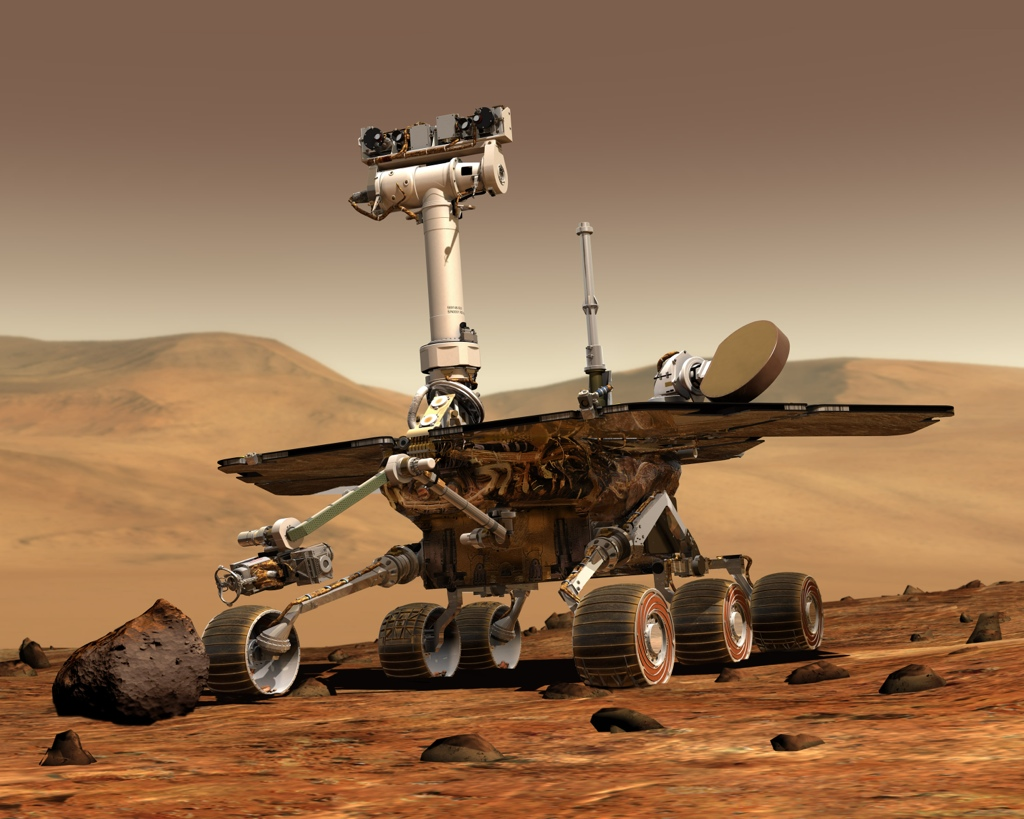
\includegraphics[width=6cm]{kapitel3/nasa_rover}
  \caption{Ein Nasa Rover}
  \label{Kap2:NasaRover}
\end{figure}

Man kann sich auch selbst ein Makro für das Einfügen von Bildern schreiben:

\bild{kapitel3/modell_point_to_point}{6cm}{Point to Point}

\begin{sidewaysfigure}
 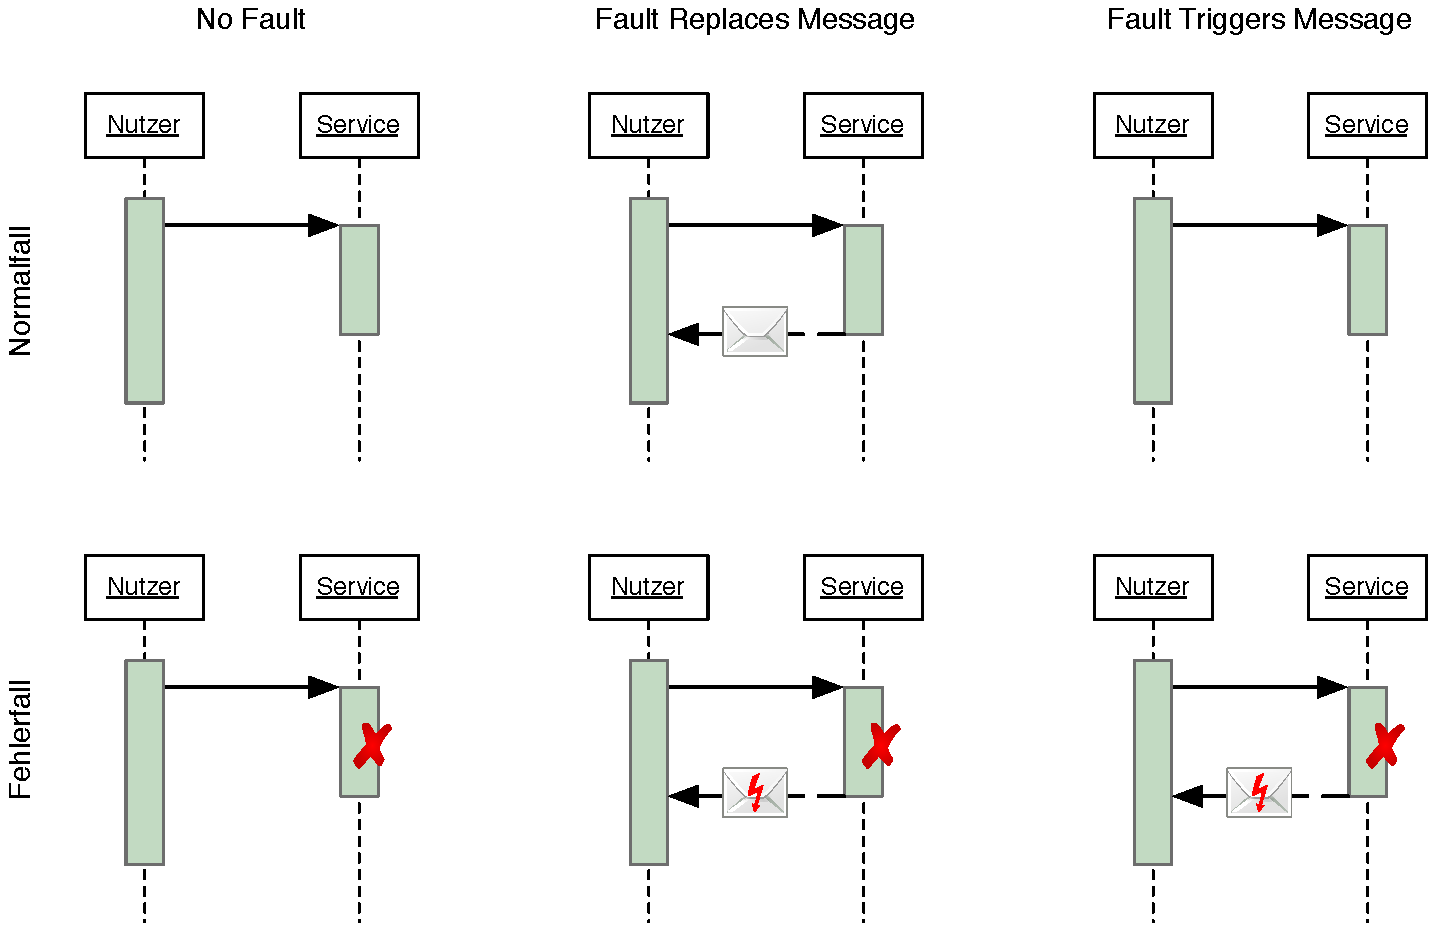
\includegraphics[width=22cm]{kapitel3/ws-wsdl20-fehler}
  \caption{Sehr große Grafiken kann man drehen, damit sie auf die Seite passen}
  \label{Kap2:wsdl-fehler}
\end{sidewaysfigure}

Möchte man verhindern, dass Bilder in ein anderes Kapitel rutschen, steht der Befehl \verb+\clearpage+ zur Verfügung, der \LaTeX{} zwingt, alle bis dahin definierten \textit{floats} (Bilder, Tabellen, Formeln etc.) auszugeben.

\clearpage % Alle Bilder, die bisher kamen ausgeben


\section{Formelsatz}

Eine Formel gefällig? Mitten im Text $a_2 = \sqrt{x^3}$ oder als eigener Absatz (siehe \autoref{Formel}):

\begin{equation}
\begin{bmatrix}
   1 &  4 &  2 \\
   4 &  0 & -3
\end{bmatrix}
        \cdot
\begin{bmatrix}
   1 &  1 &  0 \\
  -2 &  3 &  5 \\
   0 &  1 &  4
\end{bmatrix}
       {=}
\begin{bmatrix}
  -7 &  15 &  28 \\
   4 &   1 & -12
\end{bmatrix}
\label{Formel}
\end{equation}

Wenn Ihre Formel zu breit für eine Zeile wird, können Sie sie mithilfe der \texttt{split}-Umgebung und einem doppelten Backslash (\verb+\\+) umbrechen.

\begin{equation}
\label{eq:4}
\begin{split}
\mathbf{F}_{{eigen}}=\sqrt[3]{\coprod_{i=1}^{3} \lambda_{i}},
\frac{\lambda_{1}-\lambda_{3}}{\lambda_{1}},
\frac{\lambda_{2}-\lambda_{3}}{\lambda_{1}},
\frac{\lambda_{3}}{\lambda_{1}} \\-
\sum_{i=1}^{3} \lambda_{i} \log \left(\lambda_{i}\right),
\frac{\lambda_{1}-\lambda_{2}}{\lambda_{1}}
\end{split}
\end{equation}

Sie können Formelelemente auch am Gleichheitszeichen ausrichten, hierzu dient die \texttt{align}-Umgebung:

\begin{align}
2x - 5y &=  8 \\
3x + 92y &=  -12
\end{align}

Wollen Sie keine Nummerierung der Formeln, ergänzen Sie einfach einen \texttt{*} bei den Namen der Umgebungen, d.\,h. Sie verwenden \texttt{equation*} oder \texttt{align*}.

\begin{equation*}
\begin{bmatrix}
   1 &  4 &  2 \\
   4 &  0 & -3
\end{bmatrix}
        \cdot
\begin{bmatrix}
   1 &  1 &  0 \\
  -2 &  3 &  5 \\
   0 &  1 &  4
\end{bmatrix}
       {=}
\begin{bmatrix}
  -7 &  15 &  28 \\
   4 &   1 & -12
\end{bmatrix}
\end{equation*}

\section{Zahlendarstellung und Angabe von Einheiten}
Zahlen und Einheiten können wie folgt angegeben werden: 

\begin{tabular}{|l|l|}
	\hline
	\textbf{Befehl} & \textbf{Ausgabe}  \\\hline
	\verb*|\num{123}| & \num{123} \\
	\verb*|\num{1234}| &	\num{1234} \\
	\verb*|\num{12345}| &	\num{12345} \\
	\verb*|\num{0.123}| &	\num{0.123} \\
	\verb*|\num{0,12345}| &	\num{0,1234} \\
	\verb*|\num{.12345}| &	\num{.12345} \\
	\verb*|\num{3.45d-4}| &	\num{3.45d-4} \\
	\verb*|\num{-e10}| &	\num{-e10} \\
	\verb*|\qty[per-mode=symbol]{2.8}{\giga\byte\per\second}| & \qty[per-mode = symbol]{2.8}{\giga\byte\per\second}\\
	\verb*|\qty[per-mode=fraction]{2.8}{\giga\byte\per\second}| & \qty[per-mode = fraction]{2.8}{\giga\byte\per\second}\\
	\verb*|\qty[mode=text]{2.8}{\giga\byte\per\second}| & \qty[mode = text]{2.8}{\giga\byte\per\second}\\\hline
\end{tabular}

\vspace*{0.75cm}

Listen können ebenfalls mit Einheiten versehen werden:\\ \verb*|\qtylist{10;30;45}{\giga\byte\per\second}| liefert die Ausgabe: \qtylist{10;30;45}{\giga\byte\per\second}. 

Bereiche können mit dem Befehl \verb*|\qtyrange{10}{30}{\giga\byte\per\second}| ausgegeben werden. \qtyrange{10}{30}{\giga\byte\per\second}


\section{Sourcecode}

Man kann mit Latex auch ganz toll Sourcecode in den Text aufnehmen.

\subsection{Aus einer Datei}

\lstinputlisting[firstline=2,                 % Erste anzuzeigende Zeile aus der Datei
                 language=Java,               % Programmmiersprache (für Highlighting)
                 caption={Crypter-Interface}, % Beschriftung
                 label=lst:CrypterInterface]  % Label (für Referenzen)
                 {\srcloc/Crypter.java}       % Pfad zur Datei, die angezeigt wird

Mit Zeilennummern

\lstinputlisting[numbers=left,                % Mit Zeilennummern auf der linken Seite
                 firstline=10,                % Erste anzuzeigende Zeile aus der Datei
                 lastline=15,                 % Letzte anzuzeigende Zeile aus der Datei
                 language=Java,               % Programmmiersprache (für Highlighting)
                 caption={Crypter},           % Beschriftung
                 label=lst:CrypterInterface2] % Label (für Referenzen)
                 {\srcloc/Crypter.java}       % Pfad zur Datei, die angezeigt wird


\subsection{Inline}

\begin{lstlisting}[language=Java,caption=Methode checkKey()]
    /**
     * Testet den Schlüssel auf Korrektheit: Er muss mindestens die Länge 1
     * haben und darf nur Zeichen von A-Z enthalten.
     *
     * @param key zu testender Schlüssel
     * @throws CrypterException wenn der Schlüssel nicht OK ist.
     */
    protected void checkKey(Key key) throws CrypterException {

        // Passt die Länge?
        if (key.getKey().length == 0) {
            throw new CrypterException("Der Schlüssel muss mindestens " +
                    "ein Zeichen lang sein");
        }

        checkCharacters(key.getKey(), ALPHABET);
    }
\end{lstlisting}


\section{Anforderungen}

Anforderungen im Format des Volere"=Templates (Snowcards) \autocite{Volere} können per Makro eingefügt werden. Das Label wird automatisch mit der Nummer erstellt, d.\,h. Sie können auf die Tabelle mit dieser referenzieren (siehe \autoref{F52}).

\snowcard % Snowcard einbinden 
   {F52} % Nummer des Requirements
   {F} % Art
   {Hoch} % Priorität
   {User Authentifizierung} % Titel
   {Interview mit Abteilungsleiter} % Herkunft (Optional)
   {F12} % Konflikte (Optional)
   {Der Benutzer ist in der Lage sich über seinen
    Benutzernamen und sein Passwort am System anzumelden} % Beschreibung
   {Ein Benutzer kann sich mit seinem firmenweiten Benutzernamen und
   Passwort über die Anmeldemaske anmelden und hat Zugriff auf die
   Funktionen des Systems} % Fit-Kriterium (Optional)
   {Benutzerhandbuch des Altsystems} % Material (Optional)

Ebenso können Sie nicht"=funktionale Anforderungen mit Hilfe von Quality Attribute Scenarios (vgl. \autoref{NF11}) darstellen. Zu Details siehe \autocite{Barbacci2003}.

\qas % Quality-Attribute Scenario einbinden (Anpassungen in titelblatt.tex)
   {NF11} % Nummer des Requirements
   {Hoch} % Priotität
   {Performance des Jahresabschlusses} % Titel
   {Endbenutzer} % Quelle
   {Startet einen Jahresabschluss} % Stimulus
   {Buchhaltungssystem} % Artefakt
   {Das System befindet sich im normalen Betriebszustand} % Umgebung
   {Jahresabschluss ist durchgeführt und kann als PDF abgerufen werden} % Antwort
   {10 Minuten} % Antwort-Maß

Die Abgrenzung von funktionalen und nicht-funktionalen Anforderungen ist nicht immer einfach und bereitet manchen Studierenden Probleme. Als Hilfestellung kann die von der ISO25010 \autocite{ISO25010} zur Verfügung gestellte Liste dienen, siehe \autoref{kapitel3/iso25010}.

\bild{kapitel3/iso25010}{14cm}{Qualitätsmodell für Software-Produkte nach ISO25010}

\citeauthor{Bass2021} listen in \autocite{Bass2021} eine ähnliche Liste von Kategorien für nicht-funktionalen Anforderungen auf, die ebenfalls als Richtschnur dienen kann. Diese sind:

\begin{itemize}
  \item \textit{Verfügbarkeit} \textit{(availability)} -- umfasst Zuverlässigkeit (reliability), Robustheit (robustness), Fehlertoleranz (fault tolerance) und Skalierbarkeit (scalability)
  \item \textit{Anpassbarkeit} \textit{(modifiability)}, umfasst Wartbarkeit (maintainability), Verständlichkeit (understandability) und Portabilität (portability).
  \item \textit{Performanz} \textit{(performance)}
  \item \textit{Sicherheit} \textit{(security)}
  \item \textit{Testbarkeit} \textit{(testability)}
  \item \textit{Bedienbarkeit} \textit{(usability)}
\end{itemize}


\chapter{Track Changes - Manuelle Änderungsmarkierung}
In diesem Dokument können Track Changes \chreplaced[id=B1]{verwendet}{aktiviert und benutzt} werden\\ (\lstinline|\chreplaced[id=B1]{verwendet}{aktiviert und benutzt}|). Durch die ID können die Anmerkungen \chdeleted[id=B2]{einem} dem Autor zugeordnet werden (\verb|\chdeleted[id=B2]{einem}|). B1 steht für die erste betreuende Person und B2 für die zweite. Ergänzungen in einem Satz wie beispielsweise in diesem Satz \chadded[id=B1]{gibt es} kein Verb können über \lstinline|\chadded[id=B2]{gibt es}| hinzugefügt werden.  

Es ist ebenfalls möglich Textteile \chhighlight[id=B1]{hervorzuheben} mit dem Befehl \\ \lstinline|\chhighlight[id=B1]{hervorzuheben}|. Zudem können Kommentare\chcomment[id=B2]{das ist mein Kommentar} über den Befehl \lstinline|\chcomment[id=B2]{das ist mein Kommentar}| hinzugefügt werden.


Das Verzeichnis zur Ausgabe aller Änderungen erfolgt über das Flag \lstinline|tc| in der docinfo.tex.  Dieser Befehl ist vor der Abgabe unbedingt auf \lstinline|notc| zu ändern.

Weitere Informationen zu der Nutzung des Paketes finden Sie unter: \url{https://ctan.org/pkg/changes?lang=de}

\listofchanges[style=list, title=To Do's, show=all]







 % Externe Datei einbinden
\chapter{Checkliste}
\label{Kap4}

Die folgende Checkliste kann dazu dienen, die Arbeit auf die wichtigsten Bewertungskriterien zu prüfen. Jeder Dozent hat andere Kriterien, die unten aufgeführten dürften aber für die meisten Dozenten gültig sein.

\section{Form und Sprache}

\begin{checklist}
  \footnotesize
  \item \textbf{Aufbau}: Die Arbeit ist nach wissenschaftlichen Prinzipien aufgebaut (wesentliche Teile vorhanden, Nummerierung/Verweise korrekt, Verzeichnisse vorhanden).
    \begin{checklist}
        \item \textit{Wesentliche Teile}: Die folgenden Elemente der Arbeit sind vorhanden: Titelblatt, Abstract/Zusammenfassung, Einleitung, Hauptteil, Fazit/Ausblick.
        \item \textit{Nummerierung/Verweise}: Das Nummerierungsschema wird konsistent über die gesamte Arbeit durchgehalten, die Verweise auf die verschiedenen Elemente (Abbildungen, Tabellen etc.) sind korrekt.
        \item \textit{Verzeichnisse}: Die Arbeit enthält alle relevanten Verzeichnisse: Inhaltsverzeichnis, Literaturverzeichnis, Abbildungsverzeichnis, Tabellenverzeichnis, eventuell Glossar.
    \end{checklist}
  \item \textbf{Sprache}: Die verwendete Sprache entspricht wissenschaftlichen Ansprüchen.
    \begin{checklist}
        \item \textit{Begriffe und Definitionen}: Begriffe werden einheitlich und konsistent verwendet. Neue Begriffe werden definiert und mit Literatur hinterlegt.
        \item \textit{Abkürzungen}: Alle Abkürzungen werden eingeführt und erläutert. Abkürzungen werden bei der ersten Verwendung ausgeschrieben und in einem Abkürzungsverzeichnis geführt. Es werden keine unüblichen oder selbst erfunden Abkürzungen verwendet. Ein Glossar kann verwendet werden, um Begriffe noch einmal kompakt darzustellen.
        \item \textit{Rechtschreibung}: Die Arbeit ist frei von Rechtschreibungs-, Zeichensetzungs- und Grammatikfehlern.
    \end{checklist}
  \item \textbf{Formatierung, Typografie}: Die Formatierung der Arbeit ist korrekt und aus typographischer Sicht einwandfrei. \textit{Wenn Sie dieses Template korrekt verwenden, sollte dieser Punkt automatisch durch die Verwendung von \LaTeX{} erledigt sein.}
    \begin{checklist}
        \item \textit{Korrekte Typografie}: Schriftarten werden korrekt verwendet (nicht mehr als 2 Fonts), der Zeilenabstand ist passend, die Ränder sind ausreichend, der Satz ist korrekt.
        \item \textit{Satz von Abbildungen, Tabellen etc.}: Abbildungen sind in der richtigen Auflösung dargestellt, die Tabellen sind korrekt gesetzt, mathematische Formeln und Symbole sind sauber dargestellt.
    \end{checklist}
  \item \textbf{Abbildungen}: Abbildungen werden in ausreichendem Umfang zur Förderung des Verständnisses eingesetzt. Sie werden korrekt im Text referenziert und sind, wo immer möglich, in einer Standardnotation erstellt.
    \begin{checklist}
        \item \textit{Ausreichende Verwendung}: Komplizierte Sachverhalte werden durch Abbildungen verdeutlicht. Es werden genug Abbildungen eingesetzt, um die wichtigsten Sachverhalte zu erklären.
        \item \textit{Verständnisförderung}: Abbildungen dienen nicht als Schmuck, sondern um komplizierte Sachverhalte zu verdeutlichen.
        \item \textit{Einbindung in den Text}: Der Text muss auch ohne Abbildungen verständlich sein, die Abbildungen helfen Sachverhalte aus dem Text besser darzustellen. Der Text referenziert die Abbildung korrekt.
        \item \textit{Standardnotation, Legende}: Die Abbildungen verwenden Standard"=Notationen wie UML, FMC etc. Wo keine Standardnotation eingesetzt wird, ist eine Legende vorhanden, um die Bildelemente zu erläutern.
    \end{checklist}
  \item \textbf{Zitate}: Quellen werden konsistent nach einer gängigen Zitierweise zitiert und sind vollständig im Literaturverzeichnis angegeben.
    \begin{checklist}
        \item \textit{Zitierweise}: Die Zitierweise in der gesamten Arbeit folgt einem einheitlichen Schema, \zb{} IEEE, DIN, Chicago.
        \item \textit{Vollständigkeit}: Alle Zitate sind als solche kenntlich gemacht und die Quelle wird vollständig angegeben, und Plagiate werden vermieden.
    \end{checklist}
  \item \textbf{Schreibstil}: Lebendiger, wissenschaftlicher und verständlicher Schreibstil.
    \begin{checklist}
        \item \textit{Wissenschaftlichkeit}: Der Text ist im Präsenz geschrieben, es wird die dritte Person verwendet, Fachausdrücke werden korrekt verwendet, Fremdwörter und Amerikanismen werden richtig eingesetzt.
        \item \textit{Verständlichkeit}: Abschweifungen und Wiederholungen werden vermieden, statt dessen werden präzise und übersichtliche Sätze verwendet.
        \item \textit{Lebendigkeit}: Der Text der Arbeit zeichnet sich durch eine gute Wortwahl, Sprachbilder, einen angemessenen Satzbau und eine hohe Variabilität aus.
    \end{checklist}
\end{checklist}

\section{Inhalt}

\begin{checklist}
  \footnotesize
  \item \textbf{Gliederung}: Die Gliederung ist vollständig, konsistent und sachlogisch mit angemessener Struktur und Tiefe.
    \begin{checklist}
        \item \textit{Konsistenz und Vollständigkeit}: Auf einer Ebene stehen keine Punkte alleine, die Gliederungspunkte orientieren sich an der Argumentationskette.
        \item \textit{Angemessene Tiefe}: Die Größe der einzelnen Unterpunkte ist vom Umfang her ähnlich. Es gibt keine Gliederungspunkte, die nur aus ein bis zwei Sätzen bestehen.
    \end{checklist}
  \item \textbf{Grundlagen}: Es werden alle relevanten Grundlagen gelegt. Der State"=of"=the"=art und der State"=of"=practice werden dargelegt.
    \begin{checklist}
        \item \textit{Umfang}: 1/3 des Hauptteils ist ein gutes Maß für eine ausreichende Darstellung der Grundlagen.
        \item \textit{Begriffe und Methoden}: Begriffe und Methoden sind definiert, und Literatur zu den Definitionen ist angegeben.
        \item \textit{State-of-the-art}: Der Stand des verfügbaren Wissens wird dargestellt, analysiert und kritisch beurteilt (state-of-the-art). Bei theoretischen Arbeiten kann ein eigenes Kapitel \enquote{verwandte Arbeiten} nötig sein, um den state"=of"=the"=art darzustellen.
        \item \textit{State-of-practice}: Bei praktischen Arbeiten, die in der Industrie geschrieben werden, kann es nötig sein, auch das Vorgehen im Unternehmen zu erläutern.
    \end{checklist}
  \item \textbf{Methodik/Lösung}: Die gewählte Methodik bzw. Lösung ist für das Problem adäquat.
    \begin{checklist}
        \item \textit{Anforderungen an die Lösung}: Die von der Lösung zu erfüllenden Anforderungen werden dargestellt. Wo nötig wird dies auf Grundlage eines sauberen Requirements"=Engineerings durchgeführt.
        \item \textit{Erläuterung des Lösungsansatzes}: Der gewählte Lösungsansatz wird ausführlich erläutert und verständlich dargestellt.
        \item \textit{Eignung zur Lösung der Aufgabe}: Die gewählte Lösung ist geeignet, um das beschriebene Problem zu lösen.
        \item \textit{Hypothesen}: Es sind ggf. Hypothesen gebildet worden; diese sind erläutert, und es sind Kriterien identifiziert worden, mit deren Hilfe man die Hypothesen falsifizieren kann.
        \item \textit{Alternativen}: Es werden Alternativen zur vorgeschlagenen Lösung diskutiert. Die eigene Lösung wird nicht als einzige mögliche dargestellt, sondern es werden auch andere mögliche Lösungen vorgestellt und bewertet.
        \item \textit{Begründung}: Alternativen und Kriterien für die Auswahl dieser Lösung werden dargestellt.
        \item \textit{Vorteile der Lösung}: Es wird dargestellt, wieso die entwickelte Lösung vorteilhafter ist als die bisherigen Ansätze. Diese Darstellung erfolgt auf Basis des Lösungsansatzes. Eine konkrete Validierung der Implementierung erfolgt ggf. in späteren Kapiteln.
    \end{checklist}
  \item \textbf{Logik der Argumentationskette}: Die Argumentation ist logisch und nachvollziehbar. Sie ist frei von logischen Fehlschlüssen.
  \item \textbf{Implementierung}: Wenn eine Implementierung der Lösung erfolgt, so wird die Implementierung beschrieben. Die Darstellung der Implementierung kann knapp ausfallen. Wichtig ist der Lösungsansatz, nicht die konkrete Umsetzung.
  \item \textbf{Validierung}: Die vorgeschlagene Lösung wird ggf. empirisch verprobt.
    \begin{checklist}
        \item \textit{Vorgehensweise}: Die Vorgehensweise zur Validierung der Lösung / Hypothesen ist beschrieben und geeignet, relevante Aspekte der Lösung zu überprüfen.
        \item \textit{Empirische Analyse}: Die Erfassungsmethode wird dargestellt und die Daten werden nach den Grundsätzen ordnungsgemäßer Laborpraxis gesammelt und statistisch korrekt ausgewertet.
        \item \textit{Verprobung}: Die Lösung wird an einem praktischen Beispiel verprobt, und es werden wissenschaftlich korrekte Schlüsse aus der Anwendung gezogen.
        \item \textit{Zielerreichung}: Funktioniert die gewählte Lösung nach der Implementierung? Wie weit wurde das Ziel erreicht? Falls nicht, gibt es nachvollziehbare Gründe dafür und wurden diese dargestellt?
    \end{checklist}
  \item \textbf{Diskussion}: Die Lösung und ihre Validierung wird kritisch und im Kontext möglicher Alternativen diskutiert und bewertet.
    \begin{checklist}
        \item \textit{Kritische Reflexion}: Grenzen und Schwächen der eigenen Ergebnisse werden beleuchtet.
        \item \textit{Ableitung von Konsequenzen}: Die Konsequenzen aus den Ergebnissen für die Wissenschaft und Praxis sind beschrieben.
    \end{checklist}
  \item \textbf{Quellenarbeit}: Es werden hochwertige Quellen in ausreichendem Umfang genutzt und kritisch hinterfragt. Eventuell vorhandene Quellen aus dem Unternehmen werden ebenfalls berücksichtigt.
    \begin{checklist}
        \item \textit{Umfang}: Der Umfang an Quellen richtet sich stark nach Thema und Art der Arbeit. Bei einer Bachelorarbeit sind mindestens 20--30 Quellen üblich, bei einer Masterarbeit deutlich mehr.
        \item \textit{Wissenschaftliche Qualität}: Nicht zitierfähig sind Internet"=Quellen, Wikipedia"=Einträge sowie andere Bachelor- oder Masterarbeiten (sofern nicht veröffentlicht). Das ausschließliche Zitieren von Lehrbüchern ist problematisch. Aktuelle wissenschaftliche Artikel und Werke sollten in den Quellen auftauchen.
        \item \textit{Quellen \enquote{aus der Praxis}}: Wenn es im Unternehmen spezielle Quellen und Informationen gibt, so werden diese berücksichtigt, z. B. firmen- oder branchenspezifischer Informationen.
        \item \textit{Kritische Würdigung}: Quellen und Zitate werden kritisch hinterfragt und nicht einfach unreflektiert übernommen. Es gibt eine kritische Distanz bei der Quellenauswahl und Quellenauswertung.
    \end{checklist}
  \item \textbf{Fazit}: Es wird eine Zusammenfassung der Arbeit sowie Ausblick auf weitere mögliche Arbeiten im Themenfeld gegeben, etwa die Lösung ausstehender Probleme oder die Erfüllung zusätzlicher Anforderungen.
  \item \textbf{Umfang der Arbeit}: Richtgrößen: Bachelorarbeiten: 50--80 Seiten, Masterarbeiten: 60--100 Seiten, jeweils ohne Verzeichnisse und Anhang.
\end{checklist}

\section{Vor der Abgabe}

\begin{checklist}
  \footnotesize
  \item \textit{Korrektur}: Haben Sie einen Dritten die Arbeit lesen lassen und alle gefundenen Rechtschreib- und Zeichensetzungsfehler behoben?
  \item \textit{Literaturverzeichnis}: Sind im Literaturverzeichnis irrelevante Informationen entfernt? Beispielsweise bei Büchern unnötige Informationen über die Herkunft bei Google-Books oder bei Papern doppelte Angaben der DOI?
  \item \textbf{Abgabe auf Papier}
  \begin{checklist}
    \item \textit{Template passend eingestellt}: Haben Sie in der Datei \texttt{thesis.tex} eingestellt, dass Sie auf Papier abgeben wollen?
    \item \textit{Doppel- oder einseitiger Druck}: Entspricht die Einstellung des Templates dem Druck, d.\,h. ist das Template für doppelseitigen Druck eingestellt, wenn doppelseitig gedruckt werden soll und umgekehrt?
    \item \textit{Umschläge}: Sind die Umschläge vorhanden, um die Arbeit später zu binden? Die Umschläge können in der Hausdruckerei der Technischen Hochschule erworben werden.
    \item \textit{Copyshop}: Wissen Sie, wo Sie die Arbeit drucken werden? Die Hausdruckerei kann Ihre Arbeit nicht drucken.
    \item \textit{Exemplare}: Haben Sie geklärt, ob der Zweitkorrektor auch ein gedrucktes Exemplar möchte?
  \end{checklist}
  \item \textbf{Digitale Abgabe}
  \begin{checklist}
    \item \textit{Zustimmung des Betreuers/der Betreuerin}: Haben Sie mit Ihrer Betreuerin bzw. Ihrem Betreuer abgeklärt, dass Sie digital abgeben dürfen?
    \item \textit{Template passend eingestellt}: Haben Sie in der Datei \texttt{thesis.tex} eingestellt, dass Sie digital abgeben wollen?
    \item \textit{Unterschrift}: Haben Sie Ihre Unterschrift eingescannt und unter dem Namen \texttt{unterschrift.png} im Hauptverzeichnis abgelegt?
  \end{checklist}
\end{checklist}
 % Externe Datei einbinden



\label{lastpage}
%Beginn des Anhangs. Befehl \appendix nicht entfernen auch wenn kein Anhang vorhanden ist!
\appendix

%Wenn Sie keinen Anhang haben, entfernen Sie ausschließlich die nachfolgenden beiden Dateien.
\chapter{Style-Guide und Glossar}
\label{AnhangA}

% Ein PDF-Dokument laden und in dieses Dokument einbinden

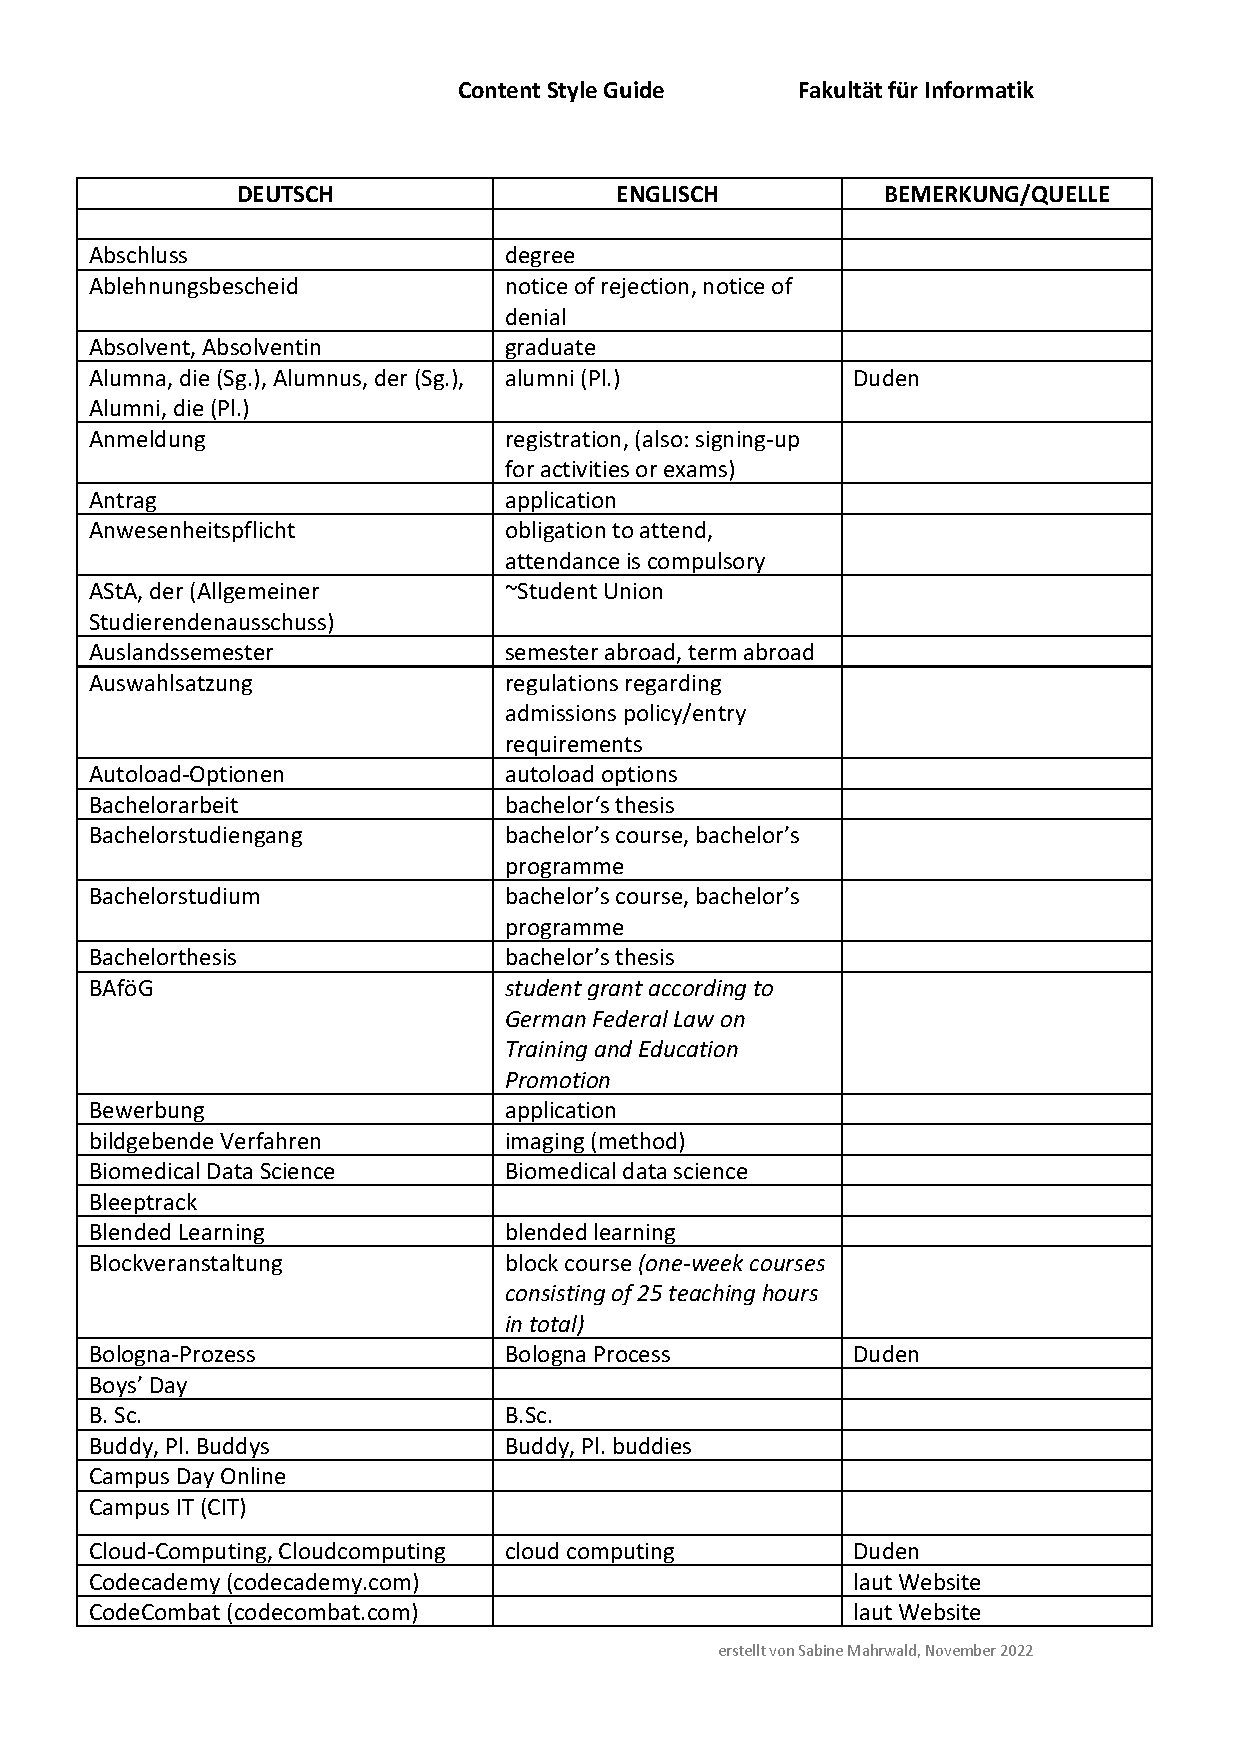
\includepdf[pages=-        % Alle Seiten des Dokumentes einbinden
           ,scale=.8      % Seiten verkleinern, damit sie zum Layout passen
           ,pagecommand={} % Layout des umgebenden Dokumentes belassen
           ]{pdfs/style_guide.pdf}

\chapter{Zweiter Anhang: Lange Tabelle}
\label{AnhangB}

Hier ein Beispiel für einen Anhang. Der Anhang kann genauso in Kapitel und Unterkapitel unterteilt werden, wie die anderen Teile der Arbeit auch.

\sffamily
\begin{footnotesize}
  \begin{longtable}[c]{ p{.5\textwidth} p{.1\textwidth} p{.1\textwidth} p{.1\textwidth}}
    \caption[Tabelle mit ISO-Ländercodes]                       % Caption für das Tabellenverzeichnis
        {Lange Tabelle mit ISO-Ländercodes\label{laendercodes}} % Caption für die Tabelle selbst
        \\
    \toprule
    \textbf{Country} & \textbf{A 2} & \textbf{A 3} & \textbf{Number} \\
    \midrule
    AFGHANISTAN                                    & AF & AFG & 004 \\
    ALBANIA                                        & AL & ALB & 008 \\
    ALGERIA                                        & DZ & DZA & 012 \\
    AMERICAN SAMOA                                 & AS & ASM & 016 \\
    ANDORRA                                        & AD & AND & 020 \\
    ANGOLA                                         & AO & AGO & 024 \\
    ANGUILLA                                       & AI & AIA & 660 \\
    ANTARCTICA                                     & AQ & ATA & 010 \\
    ANTIGUA AND BARBUDA                            & AG & ATG & 028 \\
    ARGENTINA                                      & AR & ARG & 032 \\
    ARMENIA                                        & AM & ARM & 051 \\
    ARUBA                                          & AW & ABW & 533 \\
    AUSTRALIA                                      & AU & AUS & 036 \\
    AUSTRIA                                        & AT & AUT & 040 \\
    AZERBAIJAN                                     & AZ & AZE & 031 \\
    BAHAMAS                                        & BS & BHS & 044 \\
    BAHRAIN                                        & BH & BHR & 048 \\
    BANGLADESH                                     & BD & BGD & 050 \\
    BARBADOS                                       & BB & BRB & 052 \\
    BELARUS                                        & BY & BLR & 112 \\
    BELGIUM                                        & BE & BEL & 056 \\
    BELIZE                                         & BZ & BLZ & 084 \\
    BENIN                                          & BJ & BEN & 204 \\
    BERMUDA                                        & BM & BMU & 060 \\
    BHUTAN                                         & BT & BTN & 064 \\
    BOLIVIA                                        & BO & BOL & 068 \\
    BOSNIA AND HERZEGOWINA                         & BA & BIH & 070 \\
    BOTSWANA                                       & BW & BWA & 072 \\
    BOUVET ISLAND                                  & BV & BVT & 074 \\
    BRAZIL                                         & BR & BRA & 076 \\
    BRITISH INDIAN OCEAN TERRITORY                 & IO & IOT & 086 \\
    BRUNEI DARUSSALAM                              & BN & BRN & 096 \\
    BULGARIA                                       & BG & BGR & 100 \\
    BURKINA FASO                                   & BF & BFA & 854 \\
    BURUNDI                                        & BI & BDI & 108 \\
    CAMBODIA                                       & KH & KHM & 116 \\
    CAMEROON                                       & CM & CMR & 120 \\
    CANADA                                         & CA & CAN & 124 \\
    CAPE VERDE                                     & CV & CPV & 132 \\
    CAYMAN ISLANDS                                 & KY & CYM & 136 \\
    CENTRAL AFRICAN REPUBLIC                       & CF & CAF & 140 \\
    CHAD                                           & TD & TCD & 148 \\
    CHILE                                          & CL & CHL & 152 \\
    CHINA                                          & CN & CHN & 156 \\
    CHRISTMAS ISLAND                               & CX & CXR & 162 \\
    COCOS (KEELING) ISLANDS                        & CC & CCK & 166 \\
    COLOMBIA                                       & CO & COL & 170 \\
    COMOROS                                        & KM & COM & 174 \\
    CONGO                                          & CG & COG & 178 \\
    COOK ISLANDS                                   & CK & COK & 184 \\
    COSTA RICA                                     & CR & CRI & 188 \\
    COTE D'IVOIRE                                  & CI & CIV & 384 \\
    CROATIA (local name: Hrvatska)                 & HR & HRV & 191 \\
    CUBA                                           & CU & CUB & 192 \\
    CYPRUS                                         & CY & CYP & 196 \\
    CZECH REPUBLIC                                 & CZ & CZE & 203 \\
    DENMARK                                        & DK & DNK & 208 \\
    DJIBOUTI                                       & DJ & DJI & 262 \\
    DOMINICA                                       & DM & DMA & 212 \\
    DOMINICAN REPUBLIC                             & DO & DOM & 214 \\
    EAST TIMOR                                     & TP & TMP & 626 \\
    ECUADOR                                        & EC & ECU & 218 \\
    EGYPT                                          & EG & EGY & 818 \\
    EL SALVADOR                                    & SV & SLV & 222 \\
    EQUATORIAL GUINEA                              & GQ & GNQ & 226 \\
    ERITREA                                        & ER & ERI & 232 \\
    ESTONIA                                        & EE & EST & 233 \\
    ETHIOPIA                                       & ET & ETH & 210 \\
    FALKLAND ISLANDS (MALVINAS)                    & FK & FLK & 238 \\
    FAROE ISLANDS                                  & FO & FRO & 234 \\
    FIJI                                           & FJ & FJI & 242 \\
    \bottomrule
  \end{longtable}
\end{footnotesize}
\rmfamily


\textit{Beachten Sie, dass die Tabelle manchmal erst nach dreimaligem Lauf durch \LaTeX{} richtig angezeigt wird.}



\end{document}

